\chapter{Biological Background}

In order to better understand infectious diseases from a cell biological standpoint, this chapter reviews the current state of knowledge surrounding both bacterial and viral entry mechanisms. A sweeping overview of epidemiology and pathogenesis for several specific bacterial (\textit{Bartonella henselae}, \textit{Brucella abortus}, \textit{Listeria monocytogenes}, \textit{Salmonella enterica} and \textit{Shigella flexneri}), as well as viral parasites (adenoviruses, rhinoviruses and \textit{Vaccinia virus}) is given and the chapter concludes with a look at RNA interference as this mechanism is a cornerstone of genome-wide knockdown experiments.

\section{Microbial Host-Cell Infection}

Multi-layered keratinized skin is impenetrable for almost all microbial parasites. Instead they either require breaches such as cuts, scratches, puncture wounds and arthropod bites, or environmental interfaces which offer less impervious protection. Examples include respiratory, gastrointestinal and urogenital tracts, which all contain segments where only a single layer of epithelial cells has to be overcome. Although often protected by chemical defense mechanisms (acidity of the stomach and urogenital tract, as well as microbicidal factors in mucous secretions in the respiratory tract and small intestine), combined with frequent flushing (urination, peristalsis and the coordinated beating of cilia), some microbes have adapted to survive these hostile environments.

For extracellular pathogens to successfully colonize epithelial linings, they must avoid being removed by cleansing mechanisms of the host. Many bacteria accomplish this by expressing adhesins, protein complexes that recognize and bind to specific host-cell receptors, providing host and tissue tropism. Bacterial pili serve to extend reach and penetrate mucous secretions and therefore often carry adhesins. \Gls{epec} have extended this scheme by injecting their own receptor protein \glsrev{tir} through the \glsrev{t3ss} into the host cell to which it then attaches. This has entails the additional convenience that the intracellular domain of \gls{tir} can be used to modify host cell behavior \citep{Alberts2008}.

The outside of many epithelial barriers is covered in natural bacterial flora and crossing over into sterile cavities has the advantage of not having to compete with organisms well accustomed to that particular niche. Furthermore, intracellular pathogens are no longer accessible to antibodies and phagocytic cells and perhaps have a nutrient rich environment at their disposal.

\subsection{Viral Infection Mechanisms\footnote{Much of the information presented in this chapter is compiled from the online virus encyclopedia \href{http://viralzone.expasy.org}{ViralZone}, provided by the Swiss Institute of Bioinformatics \citep{Hulo2011}.}}

The first step of any viral entering sequence is binding to the target cell surface. This can be mediated by attachment factors which simply serve to concentrate the virions on the cell surface or by virus receptors, which additionally act as communicators between host and pathogen. Common attachment factors include glycosaminoglycan chains and sialic acids and are comparatively unspecific. Glycoprotein spikes on enveloped and capsid proteins of non-enveloped viruses provide host specificity by binding cellular receptors. These cellular receptors typically serve other purposes and are exploited for infection. Binding affinity for individual interactions may be weak but aggregation of multiple interactions provide virtually irreversible avidity \citep{Smith2012}.

\paragraph{Viral import.}
For viral cell entry, different strategies exist. Enveloped viruses can either directly fuse with the plasma membrane (e.g. \gls{hiv}) or be endocytosed by the host cell (e.g. influenza), while non-enveloped viruses either create a pore and directly inject their genome into the cytosol (e.g. polio virus) or are endocytosed (e.g. adenovirus). Endocytosis has major advantages over alternative strategies. Reaching its replicatory niche within the host cell is a difficult task for a microorganism having no means of locomotion, and hijacking the endocytic system solves this problem elegantly. Furthermore, maturation of endosomes provides precise environmental cues to the invader for triggering uncoating and release. Both fusion with the cell membrane and injection of viral material into the cytosol leaves back traces of infection to be detected by the immune system. Being completely engulfed by the host, however, the intruders leave back no telltale traces. Additionally, lytic membrane penetration techniques are not as problematic to the host if only applied inside an endosome as opposed to the plasma membrane.

Endocytic viruses trigger uptake either in a receptor mediated fashion (clathrin, caveolin or lipid raft dependent) or via non-specific macropinocytosis. The clathrin pathway is most widely used, for example by rhinoviruses, some adenoviruses, and coronaviruses and presents with characteristic invaginations, termed \glspl{ccp}. The inwards facing pockets are subsequently pinched off by the membrane scission proteins dynamin-1 and dynamin-2, releasing \glspl{ccv} into the cytosol. Caveolin-mediated endocytosis is thought to be a more tightly regulated and low capacity pathway but is nevertheless exploited by several virus species, including picornaviruses and some retroviruses. Caveola formation is lipid raft dependent and recruitment of caveolin yields 50--\SI{70}{\nano\meter} flask-shaped pockets which are closed off by dynamin action. A lipid raft dependent, caveolin independent pathway has been described in simian virus 40 infection, but remains poorly understood. Lastly, larger virions such as poxviruses or herpesviruses initiate macropinocytosis, a mechanism typically employed by the cell for non-specific uptake of extracellular particles. An actin dependent membrane ruffling leads to formation of a lamellipodium which folds back onto the plasma membrane, enclosing an extraluminal volume and thus creating a macropinosome.

\begin{figure}
  \centering
  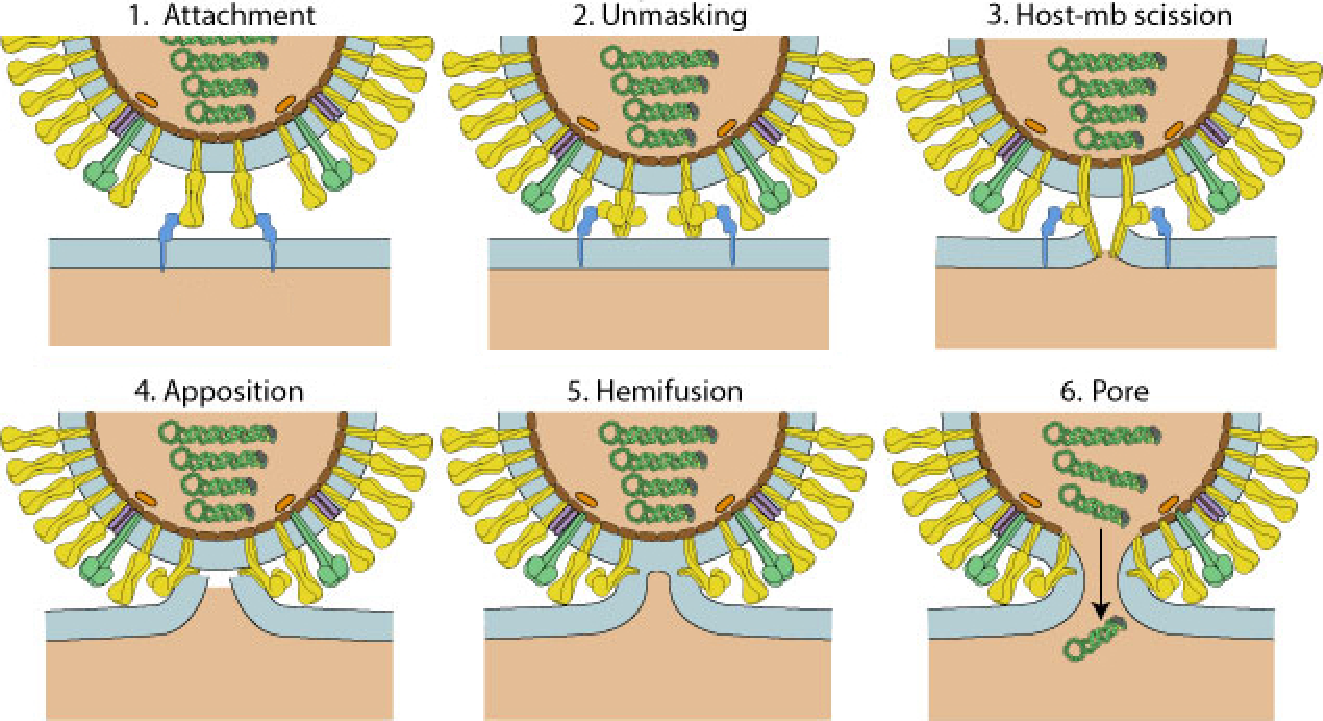
\includegraphics[width=0.95\textwidth]{virus-membrane-fusion}
  \caption[A generalized view of the steps necessary for viral--cellular membrane fusion]{A generalized view of the steps necessary for viral--cellular membrane fusion. In pre-fusion conformation, fusion proteins have their hydrophobic fusion moieties tucked away. Upon attachment (1), they are unmasked (2), interact with the target membrane and ultimately penetrate it. Conformational change in fusion proteins induces membrane scission (3) and forces the two bilayers into close proximity (4), yielding a state of hemifusion (5). Finally a fusion pore is formed (6), stabilized by the post-fusion conformation which is lower in energy than the pre-fusion state. Adapted from \cite{Hulo2011}}
  \label{fig:virus-membrane-fusion}
\end{figure}

Upon endocytic uptake, viral pathogens need to uncoat and eject their genetic material into the cytosol, as soon as their replicatory niche is reached. Escape timing is a critical issue, as late endosomes turn into lysosomes, capable of digesting their contents. Many enveloped viruses employ fusion mechanisms, which can be classified as type I or type II. For both types, increasing acidity associated with endosome maturation, initiates membrane fusion. Type I fusion proteins are forced into a metastable conformation prior to being added to the viral envelope and low pH triggers a conformational change to a state of lower energy. The energy released is used to force the two membranes close together resulting in their fusion (see figure \ref{fig:virus-membrane-fusion}). In type II fusion proteins, the critical transformation is not a conformational change but one in quaternary structure \citep{Harrison2008}.

Non enveloped viruses cannot fuse with host membranes and have developed alternative approaches such as lysis (e.g. adenovirus) or ejecting their genome through pore-forming complexes (e.g. reovirus). Polyomaviruses need to pass through the \gls{er} because they rely on \gls{er} localized proteins to uncoat their capsid. For export from the \gls{er} into the cytosol, they exploit the \gls{erad} pathway, which serves as export mechanism for misfolded proteins from the endoplasmic reticulum to be degraded by proteasomes \citep{Smith2012}.

\renewcommand{\arraystretch}{1.5}

\begin{table}
  \centering
  \caption[The Baltimore classification scheme for viruses]{The Baltimore classification scheme is based on diversity of genetic system that have evolved in viruses. For each group, a selection of virus families capable of infecting humans, is provided, along with whether the virions are enveloped and the location of their replicatory niche. The data is compiled from \cite{Hulo2011}}
  \label{tab:baltimore-classification}
  \footnotesize
  \begin{tabular}{c|llll}
    & Genome based class & Examples & Enveloped & Replication site \\
    \hline \multirow{4}{*}{\begin{sideways}DNA viruses\end{sideways}} &
    \multirow{2}{*}{Group I: dsDNA} &
    \textit{Adenoviridae} &
    no & nucleus \\
    &
    & \textit{Poxviridae} &
    yes & cytoplasm \\
    \cline{2-5} &
    \multirow{2}{*}{Group II: ssDNA(+)} &
    \textit{Parvovirinae} &
    no & nucleus \\
    &
    & \textit{Anelloviridae} &
    no & nucleus \\
    \hline \multirow{6}{*}{\begin{sideways}RNA viruses\end{sideways}} &   
    Group III: dsRNA &
    \textit{Reoviridae} &
    no & cytoplasm \\
    \cline{2-5} &
    \multirow{3}{*}{Group IV: ssRNA(+)} &
    \textit{Coronaviridae} &
    yes & cytoplasm \\
    &
    & \textit{Picornaviridae} &
    no & cytoplasm \\
    &
    & \textit{Hepeviridae} &
    no & cytoplasm \\
    \cline{2-5} &
    \multirow{2}{*}{Group V: ssRNA(-)} &
    \textit{Filoviridae} &
    yes & cytoplasm \\
    &
    & \textit{Paramyxoviridae} &
    yes & cytoplasm \\
    \hline \multirow{2}{*}{\begin{sideways}Retro\end{sideways}} &   
    Group VI: ssRNA(+)-RT &
    \textit{Orthoretrovirinae} &
    yes & nucleus \\
    \cline{2-5} &
    Group VII: dsDNA-RT &
    \textit{Hepadnaviridae} &
    yes & nucleus
  \end{tabular}
\end{table}

\paragraph{Replication.}
In contrast to larger intracellular parasites that carry the genetic information required for sustaining their own metabolism and replication, viral pathogens typically rely almost exclusively on host machinery. Furthermore, viruses have developed strategies for interfering with host transcription and translation in order to promote synthesis of viral proteins at the expense of host gene expression. Even modulation of the host cell cycle is not uncommon, as some DNA viruses (including adenoviruses) are able to trigger a G1 to S phase transition, yielding an increased concentration of active DNA polymerase, while other species are capable of inducing a G2\slash M arrest, which again provides an optimized environment for those viruses. Further virus--host interactions include regulation of apoptosis, immune response modulation and interferon signaling.

The remarkable diversity of genomic systems employed by viruses is captured by a classification system devised by \cite{Baltimore1971}. Table \ref{tab:baltimore-classification} lists the 7 types of viral genomes alongside examples of human viruses for each group, as well as whether those viruses are enveloped and where they replicate. Consequently, requirements for replication, transcription and translation vary widely among the different groups of viruses and due to the resulting mechanistic heterogeneity, viral propagation is not further explored within this general section. An excellent overview is provided by the online database of \cite{Hulo2011}.

\paragraph{Viral export.}
The final stage of the viral life-cycle is concerned with virion assembly and exiting the host cell. Again, many strategies exist. Some nuclear replicating viruses (such as polyomaviruses) assemble their capsid proteins within the nucleus, requiring their structural proteins to target the nucleus via \glspl{nls} and leave the nucleus by disrupting the nuclear envelope, while others have their genome exported via nuclear pores and assemble progeny virions in the cytoplasm. Some cytoplasmic viruses (including poxviruses) replicate within special structures called viral factories or viroplasms, which increase efficiency of assembly and packaging and provides protection from host defense mechanisms. Other cytoplasmic viruses localize to organelles such as the \gls{er} (e.g. flaviviruses) where they are assembled and enter the secretory pathway via the Golgi apparatus. For intracellular motility, large virions such as poxviruses or herpesviruses have to rely on microtubule dependent transport whereas particles smaller than \SI{20}{\nano\meter} can freely diffuse within the cytosol.

Once the host cell resources are depleted and replication is completed, progeny virions trigger their release. Viral shedding may occur via cell lysis, apoptosis, exocytosis or virion budding. Most non-enveloped and few enveloped viruses disrupt the plasma membrane with lytic viroproteins leading to cell death and release of cytoplasmic contents. While many viruses inhibit  apoptosis, typically employed as a host defense measure, some (including hepeviruses and lentiviruses) have been implicated in exploiting this mechanism for expulsion and possibly subsequent infection of macrophages. Exocytosis and virion budding are two release strategies that are non-lethal to the host cell. Enveloped viruses acquire host-derived membrane either within the cell, typically at \gls{er} or Golgi exit sites or directly from the plasma membrane. In the latter case, envelopment coincides with host exit, whereas in the former case, virions are expelled via fusion of exocytic vesicles with the plasma membrane.

\subsection{Bacterial Entry Mechanisms}

Due to the much larger size of bacterial pathogens, endocytosis is not a feasible mechanism for entry, whereas phagocytosis can deal with uptake of particles this large. While phagocytosis is a function usually only available to macrophages, some bacteria have evolved mechanisms of inducing phagocytosis in other cell types. Species explicitly targeting macrophages, such as \textit{Mycobacterium tuberculosis} and \textit{Legionella pneumophila}, have to be able to escape phagosomes or deal with resisting digestion.

Two recurring patterns for inducing phagocytosis in non-phagocytic cells have been described by \cite{Cossart2004} as zipper (encountered in \textit{Yersinia pseudotuberculosis} and \textit{Listeria monocytogenes}) and trigger mechanisms (used by \textit{Salmonella enterica} and \textit{Shigella flexneri}). Not all entry strategies can be assigned to these two classes and several additional, unrelated pathways have been uncovered.

\begin{figure}
  \centering
  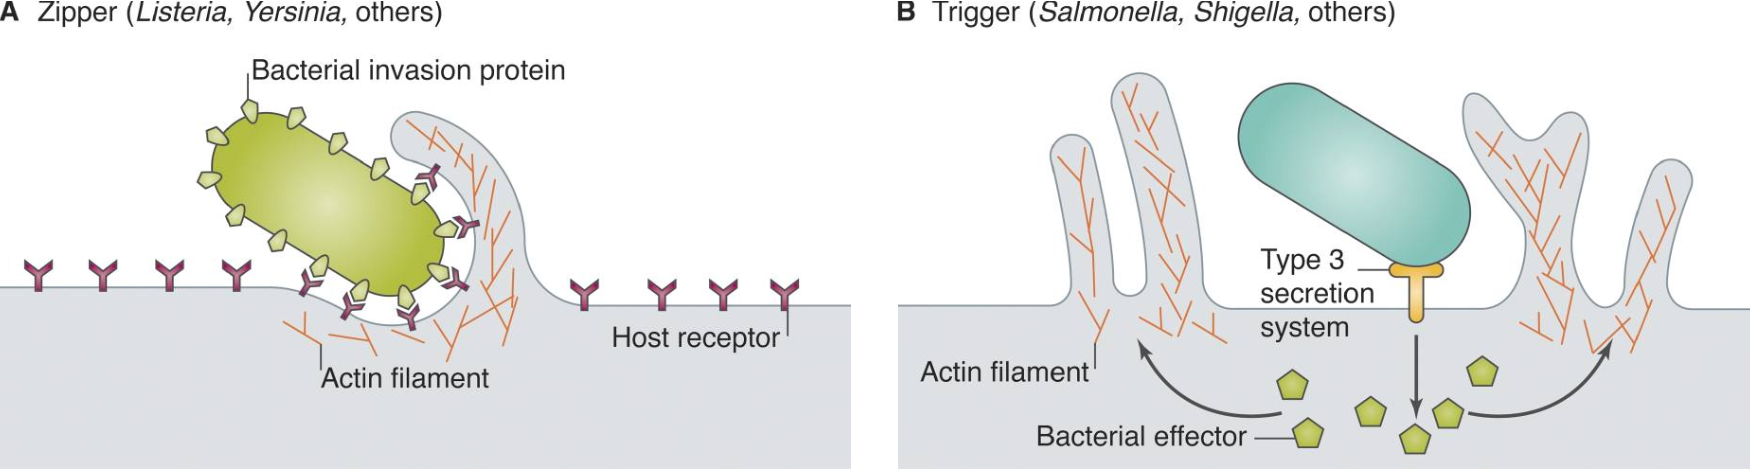
\includegraphics[width=0.95\textwidth]{zipper-trigger}
  \caption[Zipper and trigger mechanisms for bacterial host-cell entry]{Both the zipper (A) and trigger mechanisms (B) are actin dependent and lead to phagocytosis by usually non-phagocytic host cells. Zippering bacteria display an invasion protein on their surface that recruits actin filaments via a host receptor, while triggering bacteria inject an effector into the host cytosol by means of a syringe like type III secretion system leading to their uptake. Adapted from \cite{Haglund2011}.}
  \label{fig:zipper-trigger}
\end{figure}

\phantomsection
\label{zipper-mechanism}

\paragraph{Zipper mechanism.}
Host entry by zippering bacteria is characterized by bacterial surface proteins binding to cellular receptors, thereby inducing signaling cascades that lead to limited, localized actin rearrangements. This extends the plasma membrane alongside the entering bacteria in a zipper-like fashion. \citeauthor{Cossart2004} divide the scheme into three successive steps:
\begin{enumerate}[label=(\alph*)]
  \item Contact and adherence. Independent of the actin cytoskeleton, bacterial adhesins interact with host cell surface proteins leading to receptor clustering. \textit{Y. pseudotuberculosis} displays invasin, capable of interacting with \textbeta$_1$ integrins, while \textit{L. monocytogenes} uses internalin A, a protein that binds E-cadherin. Cadherin and integrins are usually involved in anchoring cell junctions and the invading bacteria mimic initiation of junction formation by a neighboring cell.
  \item Phagocytic cup formation. Responding to the mistaken signal, the target cell extends its surface towards the signal origin via \glsrev{arp23} and \glsrev{rac-1} mediated actin polymerization, attempting to cover the adhesive surface. This leads to engulfment of the invading bacterium. 
  \item Phagocytic cup closure. In a process probably involving the phosphotransferase phosphatidylinositol-4-phosphate 5-kinase, catalyzing the conversion of \glsrev{pi4p} to \glsrev{pi45p2}, the protruding membrane sections fuse and actin depolymerization returns the plasma membrane to its original state.
\end{enumerate}

\phantomsection
\label{trigger-mechanism}

\begin{table}
  \centering
  \caption[Homologous genes of \gls{t3ss} in \textit{Salmonella} and \textit{Shigella}.]{A selection of \gls{t3ss} genes in \textit{Salmonella} and \textit{Shigella}. The \textit{Salmonella} genome encodes two separate secretion systems which are deployed at distinct phases of infection. The data was obtained from \cite{Wang2012}.}
  \label{tab:t3ss-genes}
  \footnotesize
  \begin{tabular}{L{0.2\linewidth}L{0.2\linewidth}L{0.2\linewidth}L{0.2\linewidth}}
    \gls{t3ss} component&
      \textit{Salmonella} SPI-1 &
      \textit{Salmonella} SPI-2 &
      \textit{Shigella} \\
    \hline 
    Outer membrane ring &
      InvG &
      SsaC &
      MxiD \\
    Inner membrane ring &
      PrgK, PrgH &
      SsaJ, SsaD &
      MxiJ, MxiG \\
    Cytoplasmic ring &
      SpaO &
      SsaQ &
      Spa33 \\
    Export apparatus &
      % SpaR, SpaS,
      SpaP, SpaQ, InvA &
      % SsaU, SsaV
      SsaR, SsaS, SsaT &
      % Spa29, Spa40,
      Spa24, Spa9, MxiA \\
    Needle assembly &
      % OrgB
      InvI, InvJ, OrgA &
      % SsaL
      SsaO, SsaP, SsaK &
      % MxiN
      Spa13, Spa32, MxiK \\
    Needle major subunit &
      PrgI &
      SsaG &
      MxiH \\
    Needle minor subunit &
      PrgJ &
      SsaI &
      MxiI \\
    Translocon &
      SipB, SipC, SipD &
      SseB, SseC, SseD &
      IpaB, IpaC, IpaD \\
    ATPase &
      InvC &
      SsaN &
      Spa47 \\
    Effector export &
      InvE &
      &
      MxiC \\
    Chaperone &
      % SicP
      SicA, InvB, SigE &
      % SsaE
      SseA, SscA, SscB &
      % Spa15,
      IpgC, IpgE, IpgA \\
    Secreted effector &
      % AvrA, SspH1, SopD
      SipA, SptP, SopE, SopE2, SopB, SopA &
      % SspH1, SspH2, SlrP, GogB,  SseF, SseJ, SseL
      SifA, SifB, SseE, SpvC, SseG, SseI &
      % IpaH1.4, IpaH4.5, IpaH7.8, IpaH9.8, OspZ, OspB, OspF, OspC1, OspE1, OspE2, OspD1, OspG,
      IpaA, IcsB, IpgD, IpgB1, IpgB2, VirA \\
    Transcription regulator &
      % HilD, HilE, PhoP, 
      InvF, HilA, HilC, SirA, SirB, PhoP &
      SsrA, SsrB, YdgT, OmpR, H-NS, Hha &
      MxiE, VirB \\
      \hline
  \end{tabular}
\end{table}

\paragraph{Trigger mechanism.}
In trigger schemes, bacterial \gls{t3ss} weakly adhere to target cell receptors and inject effector molecules into the host cytosol through a pore formed by the syringe like delivery mechanism. These proteins directly interact with actin regulatory cellular components, causing major actin rearrangement characterized by membrane ruffling. This in turn leads to non-specific engulfment of bacteria and surrounding particles. Four steps have been identified by \citeauthor{Cossart2004}:
\begin{enumerate}[label=(\alph*)]
  \item Pre-interaction stage. Effector molecules, stored in bacterial cytosol, are associated with dedicated chaperones in order to prevent aggregation, degradation and once secretion is initiated guide them towards \gls{t3ss}. \Gls{t3ss} needle complexes (several hundred per bacterium are possible) are fully assembled and integrated into the two membranes of gram-negative bacteria.
  \item Interaction stage. The tip of \gls{t3ss} recognizes the host cell membrane and activates secretion via a process not well understood. Originally it was believed that the needle complex was able to puncture the target membrane but recent evidence suggests that translocator proteins are ejected which subsequently form a pore and thusly facilitate insertion of the secretion system. Once bacterial and cellular cytoplasms are connected, effector chaperones dissociate and unfolded proteins (the needle passage is only \SI{3}{\nano\meter} wide) enter the host in a probably \gls{atp} dependent manner. Chaperones serve a double purpose as transcription factors, encouraging synthesis of new effector protein when not attached to their substrate.
  \item Formation of macropinocytic pocket. Massive, but localized membrane protrusions emerge due to action of bacterial effectors. In \textit{Shigella} entry, VirA causes local destabilization of microtubules by binding to \textalpha\slash \textbeta-tubulin heterodimers. This in turn stimulates \glsrev{rac-1} activity, \glsrev{cdc-42} recruitment and subsequent \gls{arp23} activation leading to actin polymerization. \Acrshort{ipa}C recruits the Src tyrosine kinase further enhancing actin dynamics. \textit{Salmonella} inject the proteins \acrshort{sop}E and \acrshort{spt-p}, an activator\slash inhibitor pair for the GTPase complex \gls{rac-1}\slash \gls{cdc-42}. \Gls{gef} activity of \acrshort{sop}E induces actin rearrangements leading to formation of the macropinocytic cup.
  \item Closing of macropinocytic pocket. In \textit{Salmonella} invasion, \gls{gap} activity of \gls{spt-p}, restores the inactive \gls{gdp} state of \gls{rac-1}\slash \gls{cdc-42} and leads to actin depolymerization. Its \gls{gef} partner \acrshort{sop}E is degraded more rapidly than \gls{spt-p}, enabling reversible control over the pathways exploited for entering. In case of \textit{Shigella}, actin depolymerization is initiated by binding of \acrshort{ipa}A to vinculin, a key protein of focal adhesion plaques.
\end{enumerate}

\paragraph{Other entry pathways.}
In addition to trigger and zipper type uptake, other atypical mechanisms exist. Host cell entry of \textit{Brucella abortus}, for example, has been described as invasome mediated \citep{Dehio2005}. In this actin dependent process, bacteria aggregate on the cell surface and trigger their engulfment by injecting bacterial effectors into the host via \gls{t4ss}. The internalized structure is called an invasome.

Actin-independent uptake albeit rare, is possible as evidenced by \textit{Campylobacter jejuni} and \textit{Citrobacter freundii}, which have evolved a microtubule dependent invasion strategy \citep{Kopecko2001}. A further example of microtubule involvement is presented by \textit{Clostridium} \acrshort{spp} (a genus that includes the etiological agent of tetanus and several species capable of botulinum toxin synthesis). These intercellular pathogens induce formation of long protrusions formed by microtubule filaments that wrap around the bacteria and fix them in close proximity. It has been speculated that such a mechanism could be exploited by intracellular pathogens to promote adherence \citep{Haglund2011}.

\subsection{Intracellular Survival\footnote{Each subsection within this section is based on one or two review articles, referenced at the end of the first paragraph, respectively.}}
While bacteria that successfully subvert endocytic pathways and trigger their uptake have defied innate and evaded adaptive immune responses, they are still faced with defensive mechanisms by their new hosts. A multitude of strategies has evolved in order to undermine hostile actions directed at intruding bacteria and for establishing a replicatory niche within this initially adverse but nevertheless potentially propitious environment.

Phagocytic vacuoles, containing internalized microorganisms are destined for endocytic maturation. These compartments undergo successive acidification and finally develop into mature degradative phagolysosomes. Most intracellular pathogens either escape the endocytic vacuole before fusion with lysosomes occurs or manipulate cellular pathways that control its maturation, thereby creating a niche permissive to their survival. Two important themes for cytosolic bacteria are efficient means of locomotion and evasion of cellular responses such as autophagy \citep{Alberts2008}.

\paragraph{The phagocytic vacuole.}
In order to survive an environment characterized by constantly decreasing pH, poor nutrient content and an increasing concentration of antibacterial and lysosomal enzymes, most successful pathogens incapable of escaping their internalization compartment alter biogenesis and dynamics of their surroundings. Examples include \textit{Salmonella}, \textit{Mycobacterium tuberculosis} and \textit{Legionella pneumophila} \citep{Ham2011,Ray2009}.

\textit{Salmonella} replicates in plasma membrane derived perinuclear \glspl{scv} that are neither early, nor late endosomes. While some fusion events with vesicles of the endocytic pathway take place, maturation into lysosomes is inhibited. \Acrshort{sop}B, an \acrshort{spi}-1 encoded \gls{t3ss} effector, hydrolyzes \gls{pi45p2} and reduced concentration of \gls{pi45p2} inhibits recruitment of cellular RAB GTPases required for phagosome-lysosome fusion. A key role in manipulating membrane trafficking is played by the \acrshort{spi}-2 encoded \gls{t3ss} effector SifA. Endosomal maturation is associated with microtubule dependent vacuole relocation and SifA has been shown to regulate kinesin activity, thereby contributing to \gls{scv} integrity. Furthermore, SifA activity is essential in increasing the \gls{scv} volume and creating the necessary space for replication.

Similarly to \Acrshort{sop}B in \textit{Salmonella}, the bacterial phosphatase SapM expressed by \textit{M. tuberculosis}, dephosphorylates \gls{pi3p} which blocks phagosomes from fusing with late endosomes and consequently arrests maturation. A different approach is employed by \textit{L. pneumophila} which secrete SidC via \gls{t4ss}, an effector protein capable of binding and displaying \gls{pi4p} on the vacuolar surface. This leads to recruitment of \acrshort{er}-derived vesicles which turns the phagosome into an \glsrev{lcv} which is removed from the endocytic pathway and becomes sufficiently spacious for replication.

\paragraph{Cytosolic replication.}
Pathogens that evolved to replicate in the cytosol must quickly escape the internalization vacuole. Most species are capable of triggering their release within 30 minutes of infection, highlighting the importance of quick action in order to prevent damage incurred by acidification of the phagosome. In all known cytosolic bacteria vacuolar egress is a pathogen driven process and most species employ lytic enzymes capable of forming trans-membrane pores. Examples of bacteria that enter the cytosol as part of their life-cycle include \textit{Listeria monocytogenes}, \textit{Shigella flexneri}, \textit{Burkholderia pseudomallei}, \textit{Francisella tularensis} and species of the \textit{Rickettsia} genus \citep{Ray2009}.

The best studied organism, \textit{L. monocytogenes}, secretes \gls{llo} a hemolytic enzyme, capable of inserting into the target membrane, oligomerize and through a conformational change form a pore. This delays endosomal maturation, prevents fusion with lysosomes and finally releases the bacteria into the cytosol. Regulation of \gls{llo} is pH mediated and involves the host factor \gls{gilt}, specific to endosomes, phagosomes and lysosomes. Vacuole escape by \textit{S. flexneri} is dependent on the three \gls{t3ss} translocator proteins \gls{ipa}B, \gls{ipa}C and \gls{ipa}D with \gls{ipa}B and \gls{ipa}C forming a pore complex and \gls{ipa}D facilitating insertion into the membrane. For both \textit{Rickettsia} \acrshort{spp} and \textit{B. pseudomallei}, little information on vacuole-lytic mechanisms exist. Hemolysin C and phospholipases have been implicated of playing important roles but more work is necessary to uncover their exact mechanistic relevance. \textit{F. tularensis} stands out among the previously mentioned organisms in that lysis of the internalization vacuole is followed by re-entry of another membrane bound compartment, the \gls{fcv}.

Interestingly, it is not known to what extent, the nutritional content of mammalian cytosol is permissive to bacterial growth. As evidenced by \textit{S. flexneri} which can grow with a doubling time of only 40 minutes (growth rates in laboratory medium are comparable) it is possible for microorganisms to adapt to this environment. While it seems natural to assume that cellular cytosol provides ideal conditions for bacterial growth and replication, this raises the question of why only comparably few pathogenic organisms exploit this ecological niche. Indeed, nutritional arguments are not the only reasons to consider, as it is clear that reaching this habitat is no easy feat and further defense against foreign particles in the cytosol, for example autophagocytosis, is employed.

\begin{figure}
  \centering
  \includegraphics[width=0.95\textwidth]{actin-motility}
  \caption[Mechanisms of actin based motility in several intracellular bacterial pathogens.]{The capability for actin based motility evolved independently in several intracellular bacterial pathogens. (A) The entry points into the cellular actin assembly pathway vary, with some organisms providing their own \acrlong{npf} (\textit{Listeria} and \textit{Rickettsia}), while others rely on cellular \gls{npf} (\textit{Shigella} and \acrlong{ehec}). The branching pattern of actin tails differs between organisms relying on cellular \gls{arp23} from those capable of \gls{arp23} independent \gls{abm} (B). Cofilin is responsible for actin depolymerization, profilin is a regulatory protein catalyzing the exchange of ADP to ATP and fimbrin crosslinks actin strands into bundles. Adapted from \cite{Haglund2011}.}
  \label{fig:actin-motility}
\end{figure}

\phantomsection
\label{actin-motility}
\paragraph{\Acrfull{abm}.}
As for large viruses, free diffusion within the cytoplasm is not readily possible for bacteria and a feature common to most cytosolic bacterial is 
\gls{abm}. Actin monomers exist in two forms, G-actin (globular) and F-actin (filamentous). \Gls{atp} binds G-actin, and upon formation of a trimeric nucleus the nascent chain grows in both directions while \gls{atp} is hydrolyzed. When the chain reaches a certain length, growth becomes directional and association of monomers at the plus end compensates for dissociation of monomers at the minus end. This leads to a self-sustaining scheme described as treadmilling. Limiting to actin polymerization is the kinetically unfavorable nucleation step and in vivo, this is stimulated by cellular factors such as \gls{arp23} which require activation by \glspl{npf}, including members of the \gls{wasp} family \citep{Stevens2006,Haglund2011}.

\Gls{abm} exhibiting pathogens can be divided into two groups depending on whether they provide \glspl{npf} of their own or recruit host cell \glspl{npf}. Expression of ActA by \textit{L. monocytogenes} is both necessary and sufficient for \gls{abm} as shown in a cell free system using ActA coated beads, actin, \gls{arp23}, CapZ, cofilin and \gls{atp}. No cellular \gls{npf} is required as ActA mimics \gls{wasp} and directly activates \gls{arp23}. \textit{Rickettsia} are among the few pathogens capable of \gls{abm} without relying on \gls{arp23}, leading to formation of actin tails with a distinct morphology. The formin-like protein Sca2 directly interacts with actin and RickA, exhibiting some homology to \gls{wasp} can act as \gls{npf}. A further organism that mimics cellular \gls{npf} is \textit{B. pseudomallei}, which is capable of BimA-mediated, \gls{arp23} independent actin polymerization.

Bacterial pathogens that rely on cellular \gls{npf} instead of supplying their own include \textit{S. flexneri}, \textit{Mycobacterium marinum}  and \gls{ehec}. In \textit{S. flexneri} infection, bacterial IcsA, capable of recruiting \gls{n-wasp}, is the only required bacterial factor for triggering \gls{abm}. By inducing conformational changes in \gls{n-wasp}, IcsA is thought to mimic activation by \gls{cdc-42}, allowing for association of \gls{n-wasp} with \gls{arp23}. Details of \gls{abm} in \textit{M. marinum} are less well known but as it is both \gls{wasp} and \gls{arp23} dependent, it is assumed that the employed mechanism is similar to that of \textit{S. flexneri}.

Both \gls{ehec} and \gls{epec}, while not intracellular pathogens, are able to induce cytosolic actin polymerization. By inserting the transmembrane protein \gls{tir} into the plasma membrane they are able to initiate actin polymerization via the same pathway as \gls{abm}, leading to the formation of pedestals protruding outwards. This is thought to provide means of extracellular motility. Intercellular motility by \gls{abm} capable bacteria is achieved by pushing against the host cell membrane into the neighboring cell body until being engulfed in a double membrane vacuole that is subsequently lysed.

\phantomsection
\label{autophagy}
\paragraph{Autophagy.}
The basic catabolic cellular mechanism of autophagy is initiated as response to stress signals such as nutrient starvation, damaged cellular compartments and foreign particles. Cytoplasmic components marked for degradation are captured by the double-membrane autophagosome, intended for fusion with lysosomes. As cellular defense mechanism, cytosolic pathogens are targeted by selective autophagy in a process also related to as xenophagy. Bacterial response can be categorized as interference with the autophagy pathway, evasion of autophagy recognition or escape from the autophagosome \citep{Ham2011,Huang2014}.

\textit{S.} typhimurium, while not usually considered a cytosolic pathogen, has been shown to occasionally escape the phagocytic vacuole and replicate in the cytosol. Membrane damage triggers an amino acid starvation response that activates autophagy signaling by relocating \gls{mtor} from the late endosome to the cytosol. The bacteria respond via unknown action probably involving \acrshort{spi}-2 \gls{t3ss} secretions that are able to restore both the cytosolic amino acid pool and \gls{mtor} localization, successfully inhibiting autophagy. Further examples of autophagy-initiation signaling inhibition are provided by \textit{M. tuberculosis} which is able to produce \gls{eis}, an inhibitor to production of \gls{ros} needed as an autophagy signal. Furthermore, bacterial toxins apt to interfere with \gls{camp} regulation can block autophagy in mammalian cells.

After autophagy has been initiated, the procedure can still be modified as shown by \textit{L. pneumophila} and \textit{S. flexneri}. The former organism secretes RavZ via \gls{t4ss} which decouples the autophagy marker LC3 from the phagosomal membrane while the latter expresses VirA via \gls{t3ss}, a \gls{gap}capable of inactivating the autophagy regulator RAB1. Another group of bacteria prevent or delay lysosome fusion and accumulate in non-degradative vacuoles at neutral pH. Examples include \textit{M. marinum}, \textit{Chlamydia trachomatis}, \textit{Yersinia pestis} and \textit{Helicobacter pylori}.

Evasive measures have been suggested to be employed for \textit{S. flexneri} and \textit{L. monocytogenes}. IcsB of \textit{S. flexneri} and ActA of \textit{L. monocytogenes} have been implicated of masking the bacteria from autophagy targeting mechanisms and it has been suggested that \gls{abm} might somehow facilitate hiding from host cell detection. By also currently unknown means, \textit{B. pseudomallei} can escape the phagosome of an autophagy-related process, possibly involving BopA secretion via \gls{t3ss}.

\section{Select Bacterial Pathogens}

A total of 5 bacterial pathogens were selected for study within the InfectX \gls{rtd} project by SystemsX. This section shortly describes each organism in terms of microbiological features, pathogenesis, epidemiology and diseases caused in humans. For each organism, a chapter of \cite{Rolain2006} serves as basis and is supplemented by one or two review articles referenced in the first paragraph of each section.

\subsection{\textit{Bartonella Henselae}}

\textit{Bartonella henselae} is a short, rod shaped, unflagellated proteobacterium, phylogenetically closely related to the genus \textit{Brucella}, presenting 94.4\% 16S rRNA gene sequence homology, compared with \textit{Brucella abortus}. The Gram-negative bacillus is a facultative anaerobic, intracellular parasite and was first described in 1992. Relatively harmless for healthy humans, infections can become life threatening in immunocompromised patients, making the species an important opportunistic pathogen \citep{Anderson1997,Harms2012}.

\paragraph{Diseases.}
In immunocompetent humans, infection with \textit{B. henselae} can lead to a condition known as \gls{csd}. As the name suggests, most patients report being in contact with a cat and transmission often occurs through scratches and bites. Affecting primarily children and young adults (80\% are 21 or younger), the self limiting infection typically presents itself with lymphadenopathy. Most patients remain afebrile and do not report feeling ill, with low-grade fever and malaise shown in roughly 30\% of the cases. Recovery from uncomplicated \gls{csd} usually takes 2 to 6 months and requires no specific treatment.

Possible complications include Parinaud's oculoglandular syndrome (granulomatous conjunctivitis in one eye and parotid lymphadenitis on the same side), splenomegaly and hepatic or splenic abscesses, accompanied by fever, weight loss, fatigue and malaise. In 1 to 7\% of the cases, the disease spreads to the central nervous system, leading to encephalopathy, but recovery is usually rapid (within several weeks).

Infections with \textit{B. henselae} tend to have more severe consequences for immunocompromised patients, such as bacillary angiomatosis, bacteremia and endocarditis. \Gls{aids} patients suffering from \gls{csd} usually experience severe, progressive disease with infection spreading systematically and without appropriate treatement, fatal outcome. \textit{Bartonella} \acrshort{spp} are the only prokaryotes known to be able to induce angiogenic tumors such as bacillary angiomas, which may involve skin, respiratory or gastrointestinal epithelia, hart, liver, spleen, bone marrow, muscles, or lymph nodes. Bacteremia may lead to inflamed heart valves, usually requiring endocarditic patients to have heart valve replacement surgery.

\begin{figure}
  \centering
  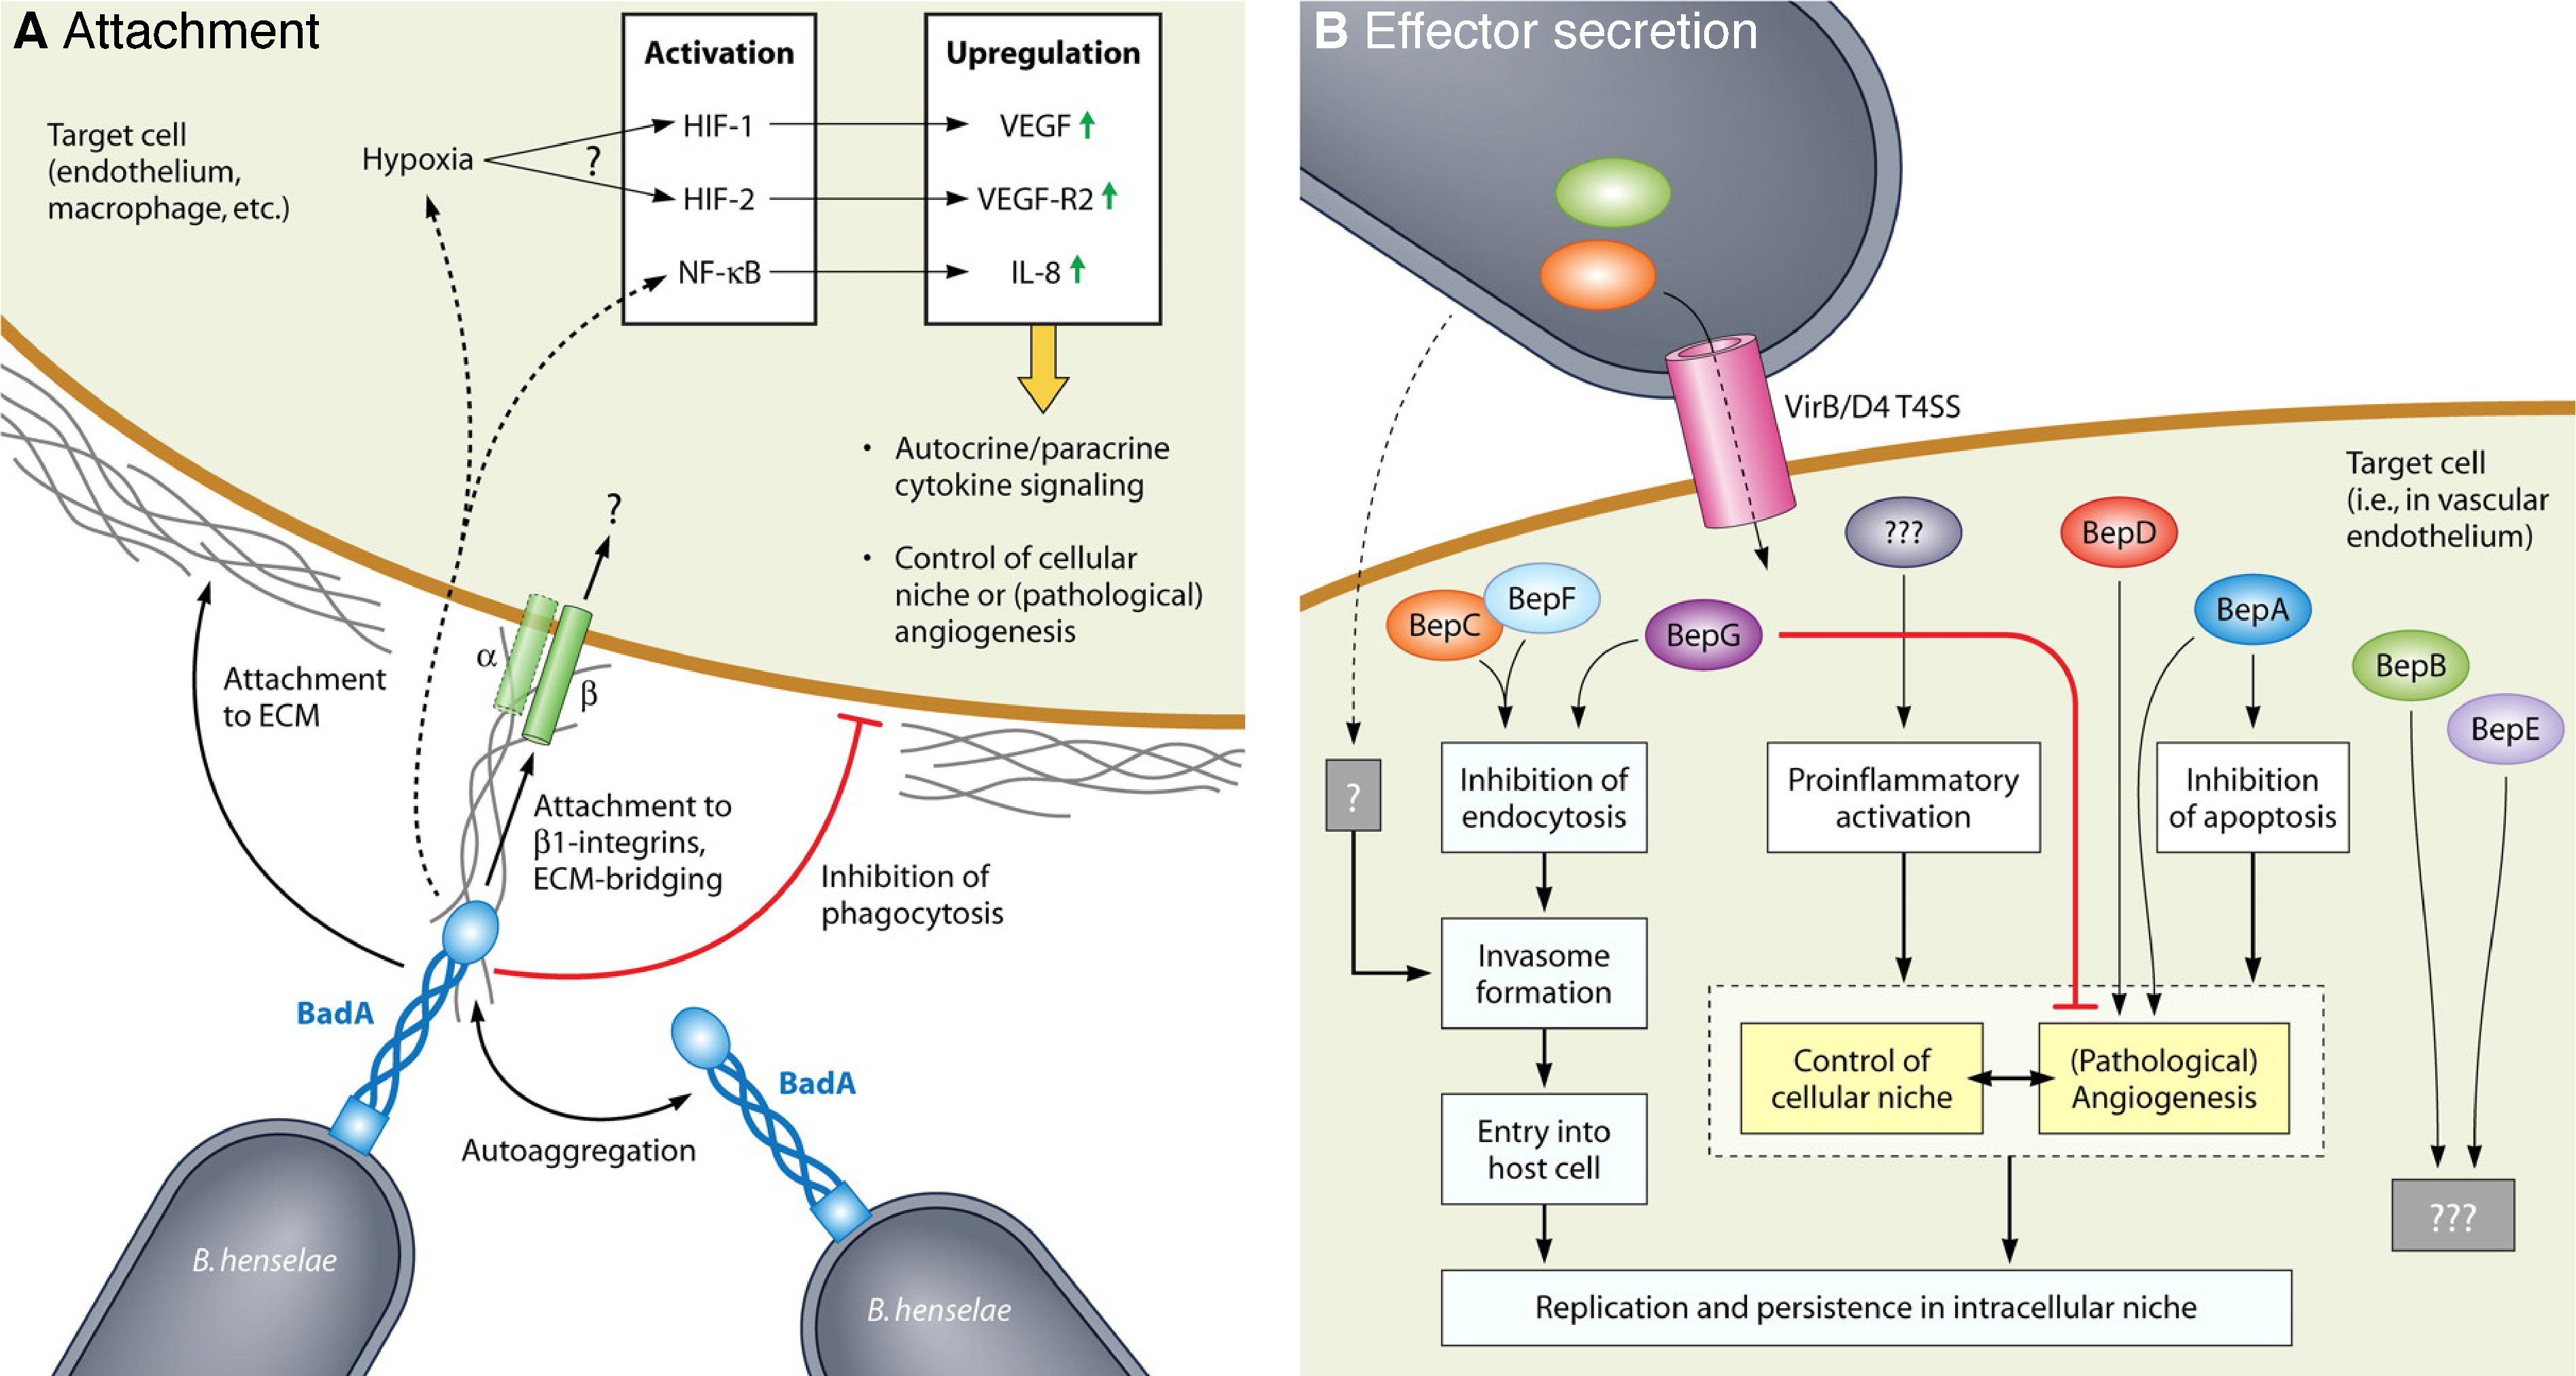
\includegraphics[width=0.75\textwidth]{bartonella}
  \caption[Bacterial effectors of \textit{B. henselae}, secreted by \gls{t4ss} into the host cytosol.]{Several effectors secreted by \gls{t3ss} in \textit{B. henselae} infection serve as virulence factors for colonization of the intracellular replicatory niche. The ones best characterized alongside their phenotype are schematically summarized. Adapted from \cite{Harms2012}.}
  \label{fig:bartonella}
\end{figure}

\paragraph{Pathogenesis.}
\textit{B. henselae} are capable of intracellular growth in both epithelial cells and erythrocytes but the focus of this section lies on infection of the former cell type. Initial attachment is mediated by the \gls{taa} BadA which is capable of both interacting with the \gls{ecm} and \textbeta$_1$-integrin, followed by effector secretion via the bacterial \gls{t4ss} VirB\slash D4. For host cell entry, two mutually exclusive mechanisms have been described. Either single bacteria or small groups are phagocytosed via a zipper-like mechanism or large clusters are internalized in a unique cellular structure termed an invasome. While invasome formation is a slow process, taking 16 to 24 hours, \glspl{bacv} resulting from endocytosis are visible within minutes. It has been suggested that inhibition of endocytosis by either a combination of effector proteins BepC and BepF or the exclusive action of BepG is crucial to invasome formation as it allows for aggregation of bacteria on the cell surface. Not the activity of effector proteins but the clustering of cellular receptors may trigger large-scale internalization (c.f. figure \ref{fig:bartonella}).

Pathological angiogenesis can be induced as the net result of a set of agonistic and antagonistic effectors. While BepG is a strong inhibitor to angiogenesis, both BepD (weakly) and BepA (strongly) promote sprouting of new blood vessels. Although the exact mechanisms of induction and regulation remain to be uncovered, the secretion of \gls{vegf} has been demonstrated in vasoproliferative tumors caused by infection with \textit{B. henselae}. Furthermore, transcriptional promotion of various factors supporting angiogenesis, including \gls{icam-1}, \gls{il-8} and angiopoietin-2 by bacterial effectors are unanimously agreed upon. Curiously, secretion of \gls{vegf} by infected endothelial cells has so far not been possible to show.

Inhibition of apoptosis is decisive to intracellular survival and it is assumed that BepA is capable of \gls{camp} mediated antiapoptotic action. The role of two further effectors that have been identified as part of the \gls{t4ss} in \textit{B. henselae}, BepB and BepE, are unknown, as are the mechanisms leading to activation of proinflammatory signalling via \glsrev{nf-kb}.

\paragraph{Epidemiology.}
The role of cats and in particular kittens, as reservoirs to \textit{B. henselae} has been firmly estabished. Infected felines are asymptomatic and show no signs of illness. Cat fleas (\textit{Ctenocephalides felis}) serve as vectors to spread the bacteria among cats and have also been suspected of infecting humans. The main path of transmission to humans however, is through scratches and bites by infected cats. \textit{B. henselae} has also been found in ticks and tick bites prior to contraction of \gls{csd} have been reported.

In the United States, 24000 cases of \gls{csd} are reported yearly, yielding 2000 hospital admissions with an estimated health care cost of \$12 million. Children are more likely to be affected (80\%) and incidence is higher in males (60\%). The seasonal pattern (occurrences higher in fall\slash winter) is attributed to cat mating patterns, as well as pet acquisition fluctuations.

\subsection{\textit{Brucella Abortus}}

The Danish physician David Bang first isolated \textit{Brucella abortus} in 1895 from cyetic cattle tissue, investigating a contagious disease causing abortions in cows. \textit{B. abortus} are small, unflagellated proteobacteria with a cell wall consisting of an outer layer (\SI{9}{\nano\meter}) of \gls{lps} and an inner layer (3--\SI{5}{\nano\meter}) of muramyl mucopeptide complexes. The Gram-negative cocobacilli appear to have evolved from free-living, soil-dwelling species and are closely related to other human pathogens such as \textit{Bartonella} \acrshort{spp}, based on 16S rRNA sequences. Brucella species were investigated for possible use as warfare agents in the mid 20th century by several armed forces. \citep{Atluri2011,VonBargen2012}

\paragraph{Diseases.}
Brucellosis is a human disease caused by several pathogenic \textit{Brucella} species, most importantly \textit{B. abortus}, \textit{B. melitensis}, \textit{B. canis} and \textit{B. suis}. Onset may be acute or insidious and due to protean symptoms, diagnosis based on clinical presentation alone is difficult. The febrile disease is generalized and may involve many parts of the body, including nervous, skeletal, gastrointestinal, cardiovascular, respiratory and genitourinary systems. Furthermore, as the bacteria spread to other reservoir hosts via their reproductive systems, persistence of infection is crucial to the pathogen and it comes as no surprise that brucellosis can manifest as a chronic disease in humans too.

\hyphenation{as-the-ni-a an-o-rex-ia nau-sea ma-laise ar-thri-tis he-p-ato-mega-ly splen-o-meg-aly epi-di-dymo-orch-it-is pul-mon-ary bron-chit-is pneu-mo-nia en-do-cardit-is men-ingit-is men-in-go-en-ceph-al-it-is}

Fever is the most consistent sign of \textit{Brucella} infection and depending on what specific organs are affected, further symptoms include asthenia, anorexia, nausea, malaise, arthritis, epididymo-orchitis in males, hepatomegaly, splenomegaly and pulmonary manifestations such as bronchitis or pneumonia. A rare complication (less than 2\%), albeit the most lethal, is infective endocarditis. Invasion of the nervous system develops in less than 5\% of cases and often results in meningitis or meningoencephalitis with good prognosis under antimicrobial treatment.

\paragraph{Pathogenesis.}
Host entry occurs primarily via the digestive system but is also possible through the respiratory tract or skin lesions. Via the gastrointestinal route, \textit{Brucella} \acrshort{spp} target Peyer's patches (lymphoid nodules localized towards the end of the small intestine) and must therefore pass through acidic conditions in the stomach. This is facilitated by expression of two ureases capable of hydrolyzing urea and producing a protective bicarbonate buffering system. When entering through the respiratory system, \textit{B. abortus} target alveolar macrophages which serve as access point to the lymphatic system therefore facilitating systematic spread.

In order to persist at systemic sites, both active and passive mechanisms for evading the immune system are in place. \Gls{lps} of the outer cell wall disguises the bacteria from \glspl{tlr} and expression of two proteins containing \gls{tir-1} domains actively interferes with \gls{tlr} signaling.

Uptake by macrophages happens via phagocytosis, which is either triggered by nonopsonized bacteria through a lipid raft mediated mechanism or by opsonization. Although opsonin marked bacteria are 10-fold more likely to be ingested, the number of pathogens reaching their destination within the host cell is higher for nonopsonized bacteria. Still, most bacteria (up to 90\%) are unsuccessful in evading their digestion and only very few are able to establish a replicative niche. Apart from professional phagocytes, epithelial cells may also be infected and the following paragraphs focus on this particular cell type.

\begin{figure}
  \centering
  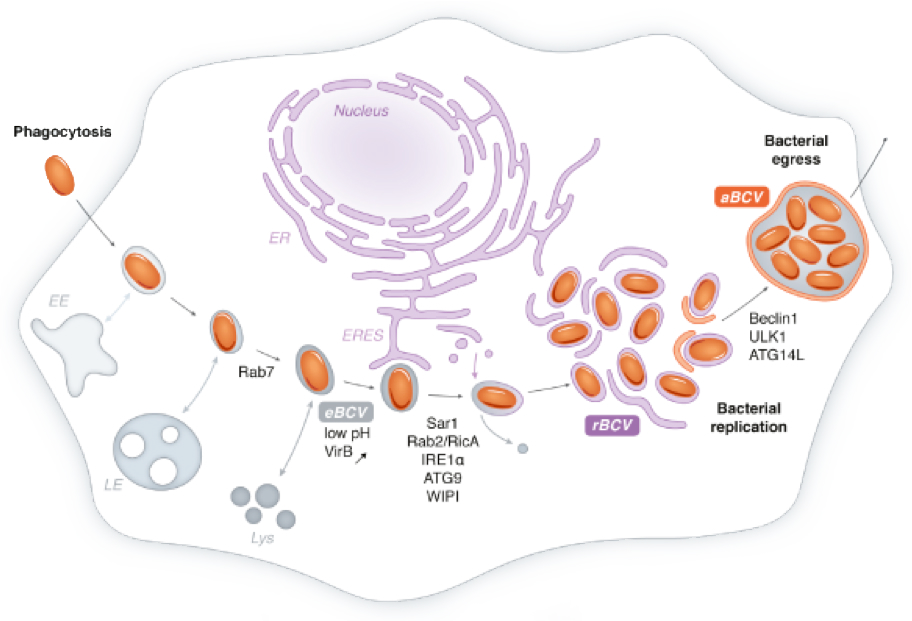
\includegraphics[width=0.75\textwidth]{brucella}
  \caption[Schematic representation of the \textit{B. abortus} intracellular life cycle.]{Schematic representation of the \textit{B. abortus} intracellular life cycle, from cell entry via maturation of the \textit{Brucella} containing vacuole to establishing an intracellular replicatory niche. Interaction with many different cellular compartments of the endocytic pathway and the \textit{cis} Golgi network are required for successful infection. Adapted from \cite{VonBargen2012}.}
  \label{fig:brucella}
\end{figure}

Initial attachment is mediated by unknown eukaryotic receptors containing sialic acid residues that interact with \gls{sp41}. While involvement of bacterial \acrshort{hsp}60 and and \gls{prpc} has been proposed, this remains controversial. Maturation of early \glspl{brcv} is important for successful infection as preventing acidification (through addition of bafilomycin A) or fusion with lysosomes (through suppression of the late-endosomal GTPase Rab7) interferes with bacterial replication. This observation can be explained with acid serving as a trigger for expression of the \gls{t4ss} VirB. However fusion events with late endosomes and lysosomes are only limited and under bacterial control.

Upon acquisition of late endosomal markers and acid initiated expression of \gls{t4ss}, fusion with autophagic vacuoles occurs, leading to formation of an autophagosome-like compartment. Subsequent interactions with \gls{er} exit sites, mediated by secreted effectors, further modify the \gls{brcv} into an \gls{er}-derived vacuole, coated with ribosomal particles. At this stage, located within the \gls{ergic}, the replicatory niche is reached. Blocking the small GTPase Sar1 inhibits intracellular replication by preventing acquisition of \gls{cop-2}, participating in anterograde \gls{er}--Golgi transport, by ER-exit vesicles. Furthermore, the small GTPase Rab2, involved in ER--cis-Golgi traffic, is required for maximal proliferation, illustrating the dependence of \textit{Brucella} on intercepting vesicular traffic.

Despite multiplying intra-cellularly in high numbers, host cells are kept alive and are even able to replicate despite infection. \textit{Brucella} species are able to interfere with apoptosis, maintaining their replicatory niche, protected from immune response. It remains unknown what happens when the hosts capacity for freeloaders is reached, as well as how bacteria exit the host cell and spread.

\paragraph{Epidemiology.}
Preferred natural reservoir species for \textit{B. abortus} are cattle (\textit{Bos taurus} and \textit{Bos indicus}) and almost all parts of the world are affected. The disease exists in both domestic and wild animals and is most prevalent in Mediterranean countries, North Africa, throughout the Middle East, India, Central Asia, as well as South and Central America. Zoonosis most often occurs through ingestion if unpasteurized milk products but airborne transmission is also possible, putting professionals involved in animal husbandry at risk. Vertical transmission among reservoir hosts can occur through lactation and horizontal transmission is facilitated by mating and placental discharge associated with aborted gestation. Human-to-human transmission is rare (but has been suspected to be possible via sexual intercourse), making humans dead-end hosts. As opposed to \textit{Bartonella}, immunodeficient patients do not seem to be especially susceptible towards \textit{Brucella} infections.

Worldwide, an estimated 500000 new cases of brucellosis occur annually, making it one of the most prevalent zoonoses. Although usually susceptible to combined antibiotic therapies of at least two agents (usually a tetracycline antibiotic combined with an aminoglycoside or rifampin), untreated brucellosis leads to a high degree of morbidity, leading to being classified a neglected zoonosis by the \gls{who}.

\subsection{\textit{Listeria Monocytogenes}}

The short, Gram-positive bacilli are non-sporeforming facultative anaerobes, capable of growing in a wide temperature range (0--\SI{50}{\celsius}) and in many different environments. Flagellation is temperature dependent with flagellin being expressed and assembled into peritrichous flagella around 20--\SI{25}{\celsius} but not at \SI{37}{\celsius}. First described in 1924 by Murray after isolation from lymph glands of diseased laboratory animals, the pathogen was found to also infect humans four years later. For much of the time since, listeriosis was considered a rare zoonotic disease and did not receive much attention. It was not until the 1980s, when several food-borne listeria outbreaks caused a shift in interest towards the pathogen, which has since become a well studied facultatively intracellular parasite \citep{Farber1991,Cossart2014}.

\paragraph{Diseases.}
Maternal and neonatal listeriosis accounts for almost half of all infections. Listeriosis in pregnancy typically manifests in bacteraemia and presents as a self-limiting febrile disease with flu-like symptoms. Many cases, however are asymptomatic and the first sign of infection is abortion or neonatal listeriosis. Maternal infection does not necessarily carry over to the fetus, especially if proper chemotherapy is administered. Perinatal incidences are divided into early and late onset (\textgreater 5 days after parturition), with former cases typically resulting in septicemia and latter cases in meningitis. While in early onset cases the predominant route of transmission is transplacental, the situation is less clear in late onset cases. Both the maternal genital tract during child birth and environmental sources have been implicated. Despite antibiotic treatment, overall mortality rates of 30--40\% are typical and prognosis for early onset disease is worse, as it is often associated with preterm birth and advanced stage of infection. 

Among adults, most cases of listeriosis occur in T-cell deficient individuals. HIV infection, for example, increases incidence 150--300 fold compared to general population control groups. Predisposing conditions include lymphoreticular neoplasms, deliberate immunosuppression (e.g. antirejection treatment after organ transplants), alcoholism and diabetes mellitus. Despite increased susceptibility caused by immunodeficiency, roughly 30\% of all infections affect immunocompetent individuals. In healthy adults, consumption of food contaminated with \textit{L. Monocytogenes} can either lead to self-limiting febrile gastroenteritis with short incubation time (\textless \SI{24}{\hour}) or invasive listeriosis with much longer incubation periods (3--4 weeks). The systemic form of infection often manifests as bacteraemia or as a neurological infection, but can also involve endocarditis and spread to other parts of the body. Central nervous system involvement occurs in as much as 75\% of cases and either presents as meningitis or encephalitis. Mortality rates of 35--45\% have been reported for listeriosis in adults.

\begin{figure}
  \centering
  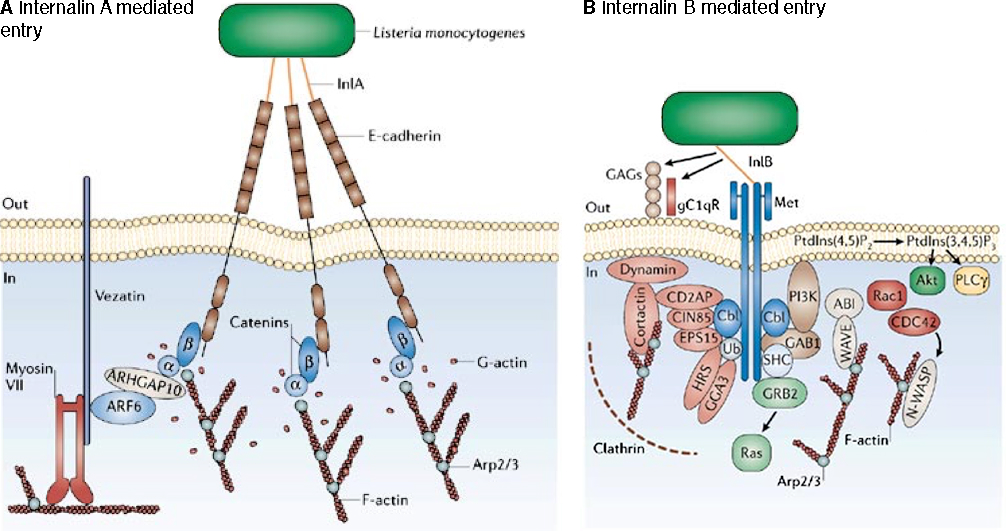
\includegraphics[width=0.95\textwidth]{listeria}
  \caption[A selection of features relevant for infection of epithelial cells by \textit{Listeria}.]{\textit{Listeria} enter host epithelial cells via a zipper-type entry mechanism mediated by the bacterial internalins InlA and InlB. In order to reach the cytosolic replicatory niche, lytic \gls{llo} is secreted and \gls{abm} provides means of locomotion. Evading host detection and maintaining a permissive environment is controlled by several bacterial effector molecules including InlC, InlK and LntA. Adapted from \citep{Cossart2014}.}
  \label{fig:listeria}
\end{figure}

\paragraph{Pathogenesis.}
The predominant entry path for \textit{L. Monocytogenes} into the human body is via the gastrointestinal tract, where Peyer's patches are targeted. The bacteria can induce cellular uptake, by non-phagocytic host cells via expression of cell-surface associated interanlins through a zipper-type entry program (see section \ref{zipper-mechanism}). The cellular receptor for bacterial internalin A is E-cadherin and internalin B interacts with the receptor tyrosine kinase c-Met. Upon internalization, the phagosomal membrane is lysed, mediated by secretion of listerial haemolysin \gls{llo} in a cholesterol dependent mechanism whereby \gls{llo} monomers associate, oligomerize and form \SI{35}{\nano\meter} pores. \gls{llo} is acid activated with an optimum around pH 5.5, which is reached in late endosomes. Moreover, \gls{llo} is required for autophagy modulation (see section \ref{autophagy}) and has been implicated in regulating inflammatory response.

Growth and replication occur in the cytoplasm and ActA mediated \gls{abm} (see section \ref{actin-motility}) provides means of intracellular and intercellular movement. Adjacent cells can be entered by pushing against the plasma membrane and forming a pseudopod-like structure which in turn is taken up the neighbor. The resulting double-membrane vacuole is escaped by cytolysis, again dependent on \gls{llo}.

Several mechanisms for persistence within the replicatory niche have recently been uncovered. Down-regulation of the host pro-inflammatory response is dependent on secretion of InlC, a virulence factor of the internalin family which prevents phosphorylation of \gls{nf-kb} and thus prevents nuclear translocation. Both InlK and ActA are associated with \gls{abm} and are simultaneously involved in autophagy evasion. Finally, mechanisms for several epigenetic host modifications have been demonstrated. Both \gls{llo} action and Met-binding during invasion, trigger histone modifications and upon entry, the virulence factor LntA localizes to the nucleus where it interacts with the newly characterized chromatin component BAHD1. While illustrating that \textit{L. monocytogenes} is capable of reprogramming host gene expression, the exact implications of this capability have yet to be elucidated.

In an extracellular setting, haemolysins serve to rupture erythrocytes in order to generate free iron, a limiting growth factor. Furthermore the nonspecific immune system has to be evaded and haemolysins have also been shown to be cytotoxic towards leukocytes. Additionally, expression of bacterial superoxide dismutase mitigates the effect of free superoxide radicals which play an important role in killing phagocytized bacteria.

\paragraph{Epidemiology.}
Incidence of listeriosis has initially been increasing since its recognition as food-borne disease but effects of awareness and diagnostic methods are unclear. While typically long incubation periods do pose difficulties for clinical diagnosis, the number of susceptible individuals is on the rise and certain aspects modern processing and handling of foods may be beneficial for growth of \textit{L. Monocytogenes}. Disease rates of 2--15 cases per million population per year have been reported and listeriosis is among the leading case of lethal food-borne pathogen infections. Most recent data, however suggests, that incidence is decreasing again.

Due to its non-fastidious lifestyle, \textit{L. Monocytogenes} has been isolated from a wire array of ecological niches, including soil, sewage and water (both fresh water bodies and estuaries). High persistence (up to 4 years) in soil samples is problematic when contaminated manure is used as fertilizer and biofilm formation poses challenges for eradication from food processing plants. Additionally, the ability to grow in refrigerated foods and resistance towards heat treatment such as pasteurization warrant alertness and special preventive care. Many different foods have been implicated in listeriosis outbreaks, including vegetables (potatoes, radishes and celery), seafood (shrimp, crabmeat and smoked fish), diary products (soft cheese, pasteurized and unpasteurized milk) and meats (poultry, various types of sausages and pâté).

Despite high prevalence in food (studies have found 20--80\% of meat product samples and 1--10\% of diary product samples contaminated with \textit{L. Monocytogenes}), comparatively few successful infections occur. The bacteria are ingested frequently in small doses and stool sample examinations suggest that 10-70\% of investigated populations could be intestinal carriers. While the minimum infectious dose has not been settled definitively, approximations range from $10^6$ to $10^9$ bacteria.

\subsection{\textit{Salmonella} Typhimurium}
\textit{Salmonella} are non-sporulating, Gram-negative bacilli, belonging to the family Enterobacteriaceae. The motile bacteria are able to produce peritrichous flagella and diameters span 0.7 to \SI{1.5}{\micro\meter} while typical lengths range from 2 to \SI{5}{\micro\meter}. They are closely related to the genus \textit{Escherichia}, showing only 15\% chromosomal sequence disparity. Currently, two distinct species, \textit{S. bongori} and \textit{S. enterica}, within the genus \textit{Salmonella} are recognized, both of which are pathogenic towards a wide array of hosts. \textit{S. enterica} is further divided into 6 subspecies, the most relevant of which for human and domestic animal hosts being \textit{enterica}. A large number of serovars (more than 2500) for \textit{S. enterica} \acrshort{subsp} \textit{enterica} have been characterized and due to an originally mistaken classification as separate species, some serovars are designated with shortened names. \textit{S.} Typhimurium, therefore is shorthand for \textit{S. enterica} \acrshort{subsp} \textit{enterica}, serovar Typhimurium and to emphasize that Typhimurium is not a species description it is not italicized.

The first description of the genus \textit{Salmonella} dates back to an investigation into swine fever led by Salmon and Smith in 1885. The newly isolated bacterium was wrongly proposed as the etiological agent, as the disease later tuned out to be caused by a virus \citep{Fabrega2013,Haraga2008}.

\paragraph{Diseases.}
Two distinct disease patterns are associated with \textit{Salmonella} \acrshort{spp} infections, typhoid fever and salmonellosis. While the former is exclusively caused by the serovars Typhi and Paratyphi, the latter is associated with several serovars, the most frequent being Enteritidis and Typhimurium, accounting for 65\% and 12\% of cases worldwide. The current and following sections will not discuss typhoid fever.

Salmonellosis is a diarrheal disease with a short incubation period of 6--24 h, followed by nausea, vomiting, loose or liquid bowel movements, abdominal cramps and fever. Clinical features are similar to those of dysentry and other gastroenteric disease and can include bloody and mucosal stool. In most cases, the infection is self-limiting and symptoms fade away within 4 to 7 days. The most common complication is bacteraemia, which presents in 5\% of cases and is more likely to develop in children, especially if malnourished, and immunocompromised individuals. Further manifestations of invasive infections include meningitis, osteomyelitis, cholangitis, pneumonia and endocarditis. While mortality in immonocompetent hosts in developed countries is as low as 0.1\%, it can increase to 77\% for \gls{hiv} positive patients in undeveloped countries.

\begin{figure}[t]
  \centering
  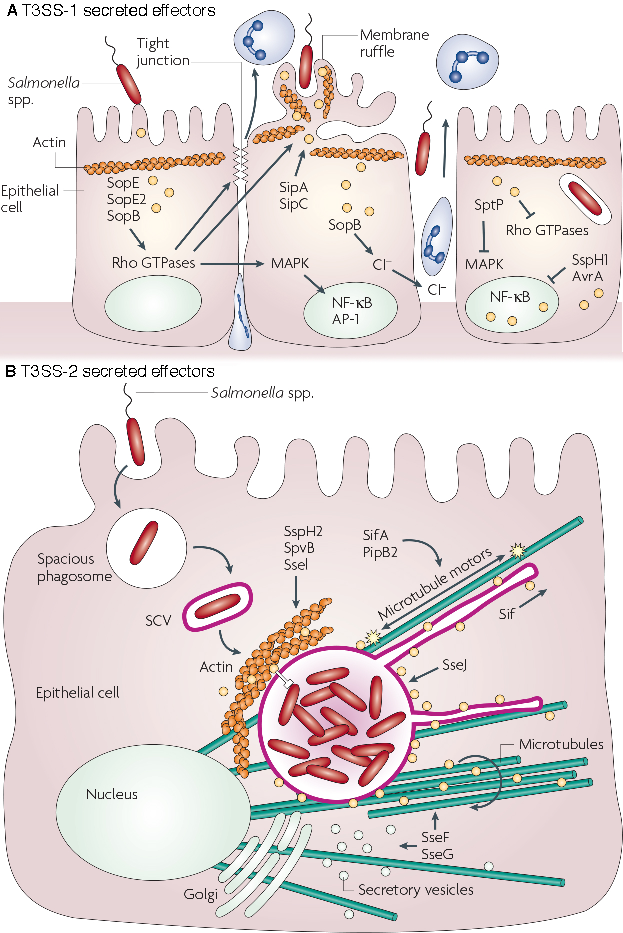
\includegraphics[width=0.7\textwidth]{salmonella}
  \caption[Overview of mechanisms for infection of epithelial cells by \textit{Salmonella} and establishing an intracellular replicatory niche.]{Two separate \gls{t3ss} are encoded in the \textit{Salmonella} genome which serve as central virulence factors at different stages of infection. \Gls{t3ss} of \acrshort{spi}-1 secretes effectors required for triggering internalization (A), while \gls{t3ss} of \acrshort{spi}-2 is critical for maturation of the phagosome into a replication permissive \gls{scv}. Figures adapted from \cite{Haraga2008}.}
  \label{fig:salmonella}
\end{figure}

\paragraph{Pathogenesis.}
In order to reach the small intestine, ingested \textit{S.} Typhimurium first have to defy the hostile environment of the stomach. A set of proteins, summarized as \gls{atr} helps mediate the acidic conditions and improves survival rates. The remaining bacteria subsequently end up in the small bowel and target epithelial cells, with preference towards \gls{m-cells}. Flagellar motility enables penetration of intestinal mucus secretions and improves the chance of reaching the intestinal walls where adhesion can be established. Fimbriae are important attachment factors, capable of interaction with host-cell laminin and fibronectin and provide an initial platform for pathogen induced phagocytosis via trigger mechanism (see section \ref{trigger-mechanism}). 

\textit{S.} Typhimurium utilize two separate \gls{t3ss} systems for host-cell colonization, the first of which (\gls{t3ss} of \acrshort{spi}-1) mediates invasion. In addition to strengthening initial interactions attaching the pathogen to its target, the needle like structure serves as delivery mechanisms, capable of injecting effector proteins, including \acrshort{sop}E, \acrshort{sop}E2, \acrshort{sop}B (also known as SigD) and \gls{sip}A. \Acrshort{sop}E serves as \gls{gef} and activates Rho GTPases \gls{rac-1} and \gls{cdc-42} via \acrshort{gdp}\slash \acrshort{gtp} exchange, which in turn initiate cytoskeletal rearrangements. \Acrshort{sop}E2 is a further \gls{gef}, highly homologous to \acrshort{sop}E and it is assumed to provide some level of redundancy for \acrshort{sop}E as shown by \textit{Salmonella} strains missing the \acrshort{sop}E gene. \Acrshort{sop}B is a phosphatase, capable of hydrolyzing various substrates, including \gls{i13456p5}, which has been linked to intestinal fluid secretion causing diarrhea and \gls{pi45p2}, involved with membrane rigidity. 

The actin binding proteins \gls{sip}A and \gls{sip}C stimulates actin polymerization and promotes membrane ruffling, yielding a macropinocytic pocket. \Glspl{mapk} initiate pro-inflammatory response via \gls{nf-kb} signaling, leading to the expression of \gls{il-8}. Furthermore, damage the tight junctions make the epithelial barrier permissive to bi-directional leakage. After internalization, actin structure is restored and \gls{mapk} signaling down regulated by SptP, SspH1 and AvrA.

Upon engulfment, maturation of the phagosome and fusion with lysosomes have to be prevented. Unlike other pathogens that escape the digestive mechanisms of phagocytic vesicles by moving to the cytosol, \textit{Salmonella} replicate inside phagosome-derived \glspl{scv}. In this setting, the second translocation complex (\gls{t3ss} of \acrshort{spi}-2) is activated, and used to secrete effectors, including SsaB and SifA, capable of interacting with vesicular trafficking mechanisms and guiding the \gls{scv} away from its original degradation pathway. Furthermore \gls{t3ss}-2 translocated effectors such as SspH2, SpvB and Ssel induce actin polymerization events, which relocate the \gls{scv} toward a perinuclear position. A last step in creating the intracellular niche needed for replication, is formation of \glspl{sif}, extending outwards from the \gls{scv}. \Gls{t3ss}-2 secretes effectors such as SifA, PipB2, SseF and SseG, which mediate the microtubule dependent processes by bundling and accumulating filaments and regulating microtubule motor function.

\paragraph{Epidemiology.}
The global disease burden caused by nontyphoidal salmonellosis is estimated at 90 million cases per year and 150000 deaths. Incidence rates are highest in East and Southeast Asia (up to 4000 cases per 100000 population per year) and both developed and undeveloped countries are affected (incidence rates in Africa are estimated at 320 while estimates for Europe are around 690 cases per 100000 population per year). An estimated 80.3 million or 86\% of reported cases are food borne \citep{Majowicz2010}.

In order to control \textit{Salmonella} outbreaks, preventive measures in food production and processing is of major importance. This starts with disease containment in domestic animals, such as vaccination of chickens, enforcing  hygiene standards in manufacturing and distribution facilities and ends with proper preparation, exploiting heat sensitivity of the organisms. As the main route of transmission is fecal--oral, good sanitary infrastructure, treatment of sewage and water processing are crucial prerequisites in combating outbreaks of salmonellosis.
% minimum infectious dose + biofilm formation leading to asymptomatic presistence

\subsection{\textit{Shigella Flexneri}}
Shigellae are small, non-sporeforming, Gram-negative bacilli and belong to the family \textit{Enterobacteriaceae}, along with \textit{Escherichia}, \textit{Salmonella} and \textit{Yersinia}. While flagellar genes are present and their expression is observed under certain conditions, the bacteria are usually described as non-motile and unflagellated. The facultative intracellular parasite shows strong specificity towards human hosts where it typically infects the lower gastrointestinal tract.

\textit{Shigella dysenteriae} was identified as the etiological agent of dysentery by Shiga in 1897 during an epidemic in Japan with 91000 reported cases and a \textgreater 20\% mortality rate. \textit{S. Flexneri} was first described by Flexner in 1900, while investigating diseases endemic to the Philippines. Recent genetic studies suggest, that \textit{Shigella} \acrshort{spp} belong to the species \textit{Escherichia coli}, rather than forming a distinct genus, as only marginal sequence divergence (1.5\%) between \textit{E. coli} and \textit{S. Flexneri} was found \citep{Schroeder2008,Croxen2010}.

\paragraph{Diseases.}
Bacillary dysentery is an acute infection of the intestine. Mild cases of the disease are self-limiting and afebrile with diarrhea and possibly vomiting as the only symptoms. In as little as 24 hours after onset, bowel movements usually begin to normalize and the condition is resolved within a few days. More severe cases are accompanied by strong abdominal cramps, fever and watery diarrhea containing blood and mucus, indicative of injury to the intestinal epithelium. While still usually self limiting in healthy individuals, recovery takes 10--14 days and relapses are possible. In immunocompromised patients, young children, especially if malnourished, and elderly individuals, life threatening complications including bacteraemia, renal failure, intestinal perforation and toxic megacolon are more frequent. Involvement of the central nervous system and respiratory tract is rare.

Administration of antibiotics is not recommended in mild to moderate cases as the disease can usually be overcome by the immune system and \gls{amr} in Shigellae is becoming an increasing concern. Oral rehydration therapy is the most effective treatment, helping the body replenish liquids and salts lost due to diarrhea. For severe infections, the use of antibiotics can become necessary and testing for resistance patterns, if possible, is advised.

\begin{figure}
  \centering
  \includegraphics[width=0.95\textwidth]{shigella}
  \caption[Route of infection and intracellular life-cycle of \textit{S. flexneri}.]{\textit{S. flexneri} cross the epithelial barrier of the distal ileum and colon by transcytosis via M cells, followed by escape from macrophage digestion. Internalization into epithelial cells from the basolateral side is mediated by trigger mechanism endocytosis. Several bacterial effectors are instrumental in reaching the replicatory niche and ensuring host survival. Adapted from \cite{Croxen2010}.}
  \label{fig:shigella}
\end{figure}

\paragraph{Pathogenesis.}
Main targets of \textit{S. Flexneri} are mucosa of the distal ileum and colon where they enter epithelial cells from the basolateral side. For initial crossing over from the apical side, action of \gls{m-cells} at Peyer's patches is exploited. These specialized enterocytes constantly sample antigens from the gut lumen and pass them to intraepithelially located dendritic cells and lymphocytes. Upon uptake by basolaterally located macrophages, \textit{S. Flexneri} survive digestive action of the phagosomal vacuole by disrupting the surrounding membrane and initiating host-cell apoptosis, mediated by the bacterial effector protein \acrshort{ipa}B, capable of acting on a caspase 1 regulated apoptotic pathway (c.f. figure \ref{fig:shigella}). The bacteria are subsequently released into the sub-mucosa, where they induce phagocytosis by normal epithelial cells via trigger mechanism (see section \ref{trigger-mechanism}).

Initial contact between pathogen and target host cell is mediated by cellular \textalpha\textsubscript{5}\textbeta\textsubscript{1} integrins and binding of \acrshort{ipa}B to CD44 receptors may initiate first actin rearrangements, preparing the cell for uptake. Subsequent injection of at least 6 effector proteins into the epithelial cytosol through the \gls{t3ss} triggers engulfment of the bacterium in an actin dependent process, involving the small GTPases \gls{rac-1} and \gls{cdc-42}, which recruit the actin nucleation complex \gls{arp23}. \Acrshort{ipa}C, a component of the translocation complex, is involved in stimulating \gls{rac-1} and \gls{cdc-42} GTPase activity through an unknown mechanism and the secreted effector proteins IpgB1, IpgB2, IpgD and \acrshort{ipa}A facilitate actin polymerization. IpgD, an inositol phosphate phosphatase, catalyzes the hydrolysis of \acrshort{pi45p2} to \acrshort{pi5p} which promotes disassociation of cytoskeleton and membrane, increasing actin availability and making the plasma membrane more susceptibility to manipulation. The mechanism of action of IpgB2 remains to be resolved, while IpgB1 is assumed to mimic activated \glsrev{rho-g}, a small GTPase, located upstream in the signaling pathway of \gls{rac-1}. Finally, binding of \acrshort{ipa}A to vinculin induces depolymerization of actin, which is assumed to be important for closing of the phagocytic cup.

The resulting phagocytic vacuole has to be escaped before maturation progresses, which is accomplished in a non-acid dependent fashion, by the translocator proteins \acrshort{ipa}B, \acrshort{ipa}C and \acrshort{ipa}D via membrane lysis. With release into the epithelial cytosol, the replicatory niche of \textit{S. Flexneri} is reached. Actin mediated intracellular motility enables intercellular dissemination (see section \ref{actin-motility}) and targeting of epithelial tight junctions initiates break-down of the epithelial barrier, providing more pathogens with access to the basolateral side of the gut lining.

\Gls{abm}, is driven by activity of two bacterial proteins. VirA is secreted at the forward facing end of the rod shaped bacilli, which promotes degradation of tubulin structures and therefore clearing a path through the dense network of microtubules and surface bound \acrshort{ics}A (\acrlong{ics} A, also referred to as VirG) facilitates actin polymerization at the opposite end. Both \gls{arp23} and \gls{n-wasp} are involved in actin nucleation, the directed nature of which provides the driving force for locomotion.

In order to maintain their intracellular niche, several strategies have evolved within the \textit{Shigella} infectome. Autophagy is inhibited by IscB (see section \ref{autophagy}) and via the previously mentioned phosphatase action of IpgD, cellular Akt proteins are activated which regulate cell survival and inhibit apoptosis. Furthermore, IpaD interacts with cell cycle regulatory protein MAD2L2, mediating cell cycle arrest. Together with OspE action on \gls{ilk}, downregulating cell detachment, this prevents turnover of epithelial cells. Inflammatory response is muddled by a combination of at least four bacterial effectors. Cytoplasmically acting OspG inhibits \gls{nf-kb}, while nuclearly located IpaH and OspB reduce \gls{il-8}. Adding to that, OspF dephosphorylates \glspl{mapk} that are required for transcription of genes of the \gls{nf-kb} pathway.

\paragraph{Epidemiology.}
Estimates by the \gls{who} peg the disease burden caused by \textit{Shigella} \acrshort{spp} at 80 million annual cases worldwide, leading to 700000 deaths. Developing countries are disproportionately affected, representing 99\% of all cases, as are children less than 5 years old, accounting for 70\% of cases and 60\% of deaths. In developed countries, incidence rates of 1--2 per 100000 population are typical and Shigellae are common causes of Traveler's diarrhea.

The predominant route of transmission is fecal--oral, highlighting the importance of sanitary precautions for infection control. Proper treatment of fecal matter is important for preventing contamination of drinking water and inhibiting spreading by disease vectors such as house flies. During acute phases, diseased individuals excrete pathogens in large numbers and as few as 100--200 organisms are sufficient of causing a new infection.

\section{Select Viral Pathogens}

In addition to the previous 5 bacterial pathogens, 3 viruses were selected for study within the InfectX \gls{rtd} project by SystemsX. This section shortly describes each pathogen in terms of physical features, pathogenesis, epidemiology and diseases caused in humans. For each section, a chapter of \cite{Craighead2000} serves as basis.

\subsection{Adenoviruses}
The family \textit{Adenoviridae} encompasses 5 genera of non-enveloped, medium sized (\SI{90}{\nano\meter} diameter) viruses, capable of infecting a broad range of vertebrate hosts. The capsid is of $T=25$ icosahedral symmetry, composed of 720 hexons arranged as 240 trimers which form the triangular facets and 12 penton capsomeres located at the vertices. A homotrimeric fiber glycoprotein protrudes from each vertex, attached to the penton base via interactions of its N-terminal domains and ending in a globular, C-terminal knob. The genome is present as double stranded DNA (Baltimore group I), is non-segmented, linear, 35--\SI{35}{\kilobase} long and encodes 40 proteins.

Adenoviruses were first isolated from human adenoid tissue cultures by Rowe in 1953 and their study led to the discovery of alternative splicing in 1977, a commonly encountered phenomenon among eukaryotes. Currently, 57 serovars are recognized as pathogenic towards humans, all belong to the genus \textit{Mastadenovirus} and are classified into 6 species, labeled A through G. The following sections are mostly concerned with \textit{Human adenovirus C} \citep{Lenaerts2008}.

\paragraph{Diseases.}
In immunocompetent individuals, adenoviruses seldom cause more than transient disease with many infections even occurring subclinically and fatal outcome being very uncommon. Symptomatic cases usually manifest as respiratory tract infections or conjunctivitis and less frequently as hemorrhagic cystitis, nephritis or gastroenteritis. Infections of the oropharynx can spread to the lower respiratory tract, causing bronchitis, bronchiolitis or pneumonia, which can become chronic, leading to desquamated epithelial tissue and long-term damage to the respiratory mucosa. Heart failure and central nervous system involvement can occur in severe cases. Ocular infections range from mild, short-term follicular conjunctivitis to highly contagious keratoconjunctivitis with possible long-term damage to the cornea. \textit{Human adenovirus C} serotypes are mostly associated with respiratory diseases but have also been implicated in eye infections.

Invasive forms of disease are mostly limited to immunocompromised individuals, including transplant recipients, \gls{hiv} infected, hereditary immunodeficient and cancer patients subject to chemotherapy. In addition to the lungs, a wide variety of organs has been reported to be affected, such as partoid glands, liver, gall bladder, colon, brain and kidney and pathological changes range from perivascular cuffing to parenchymal necrosis.

\begin{figure}
  \centering
  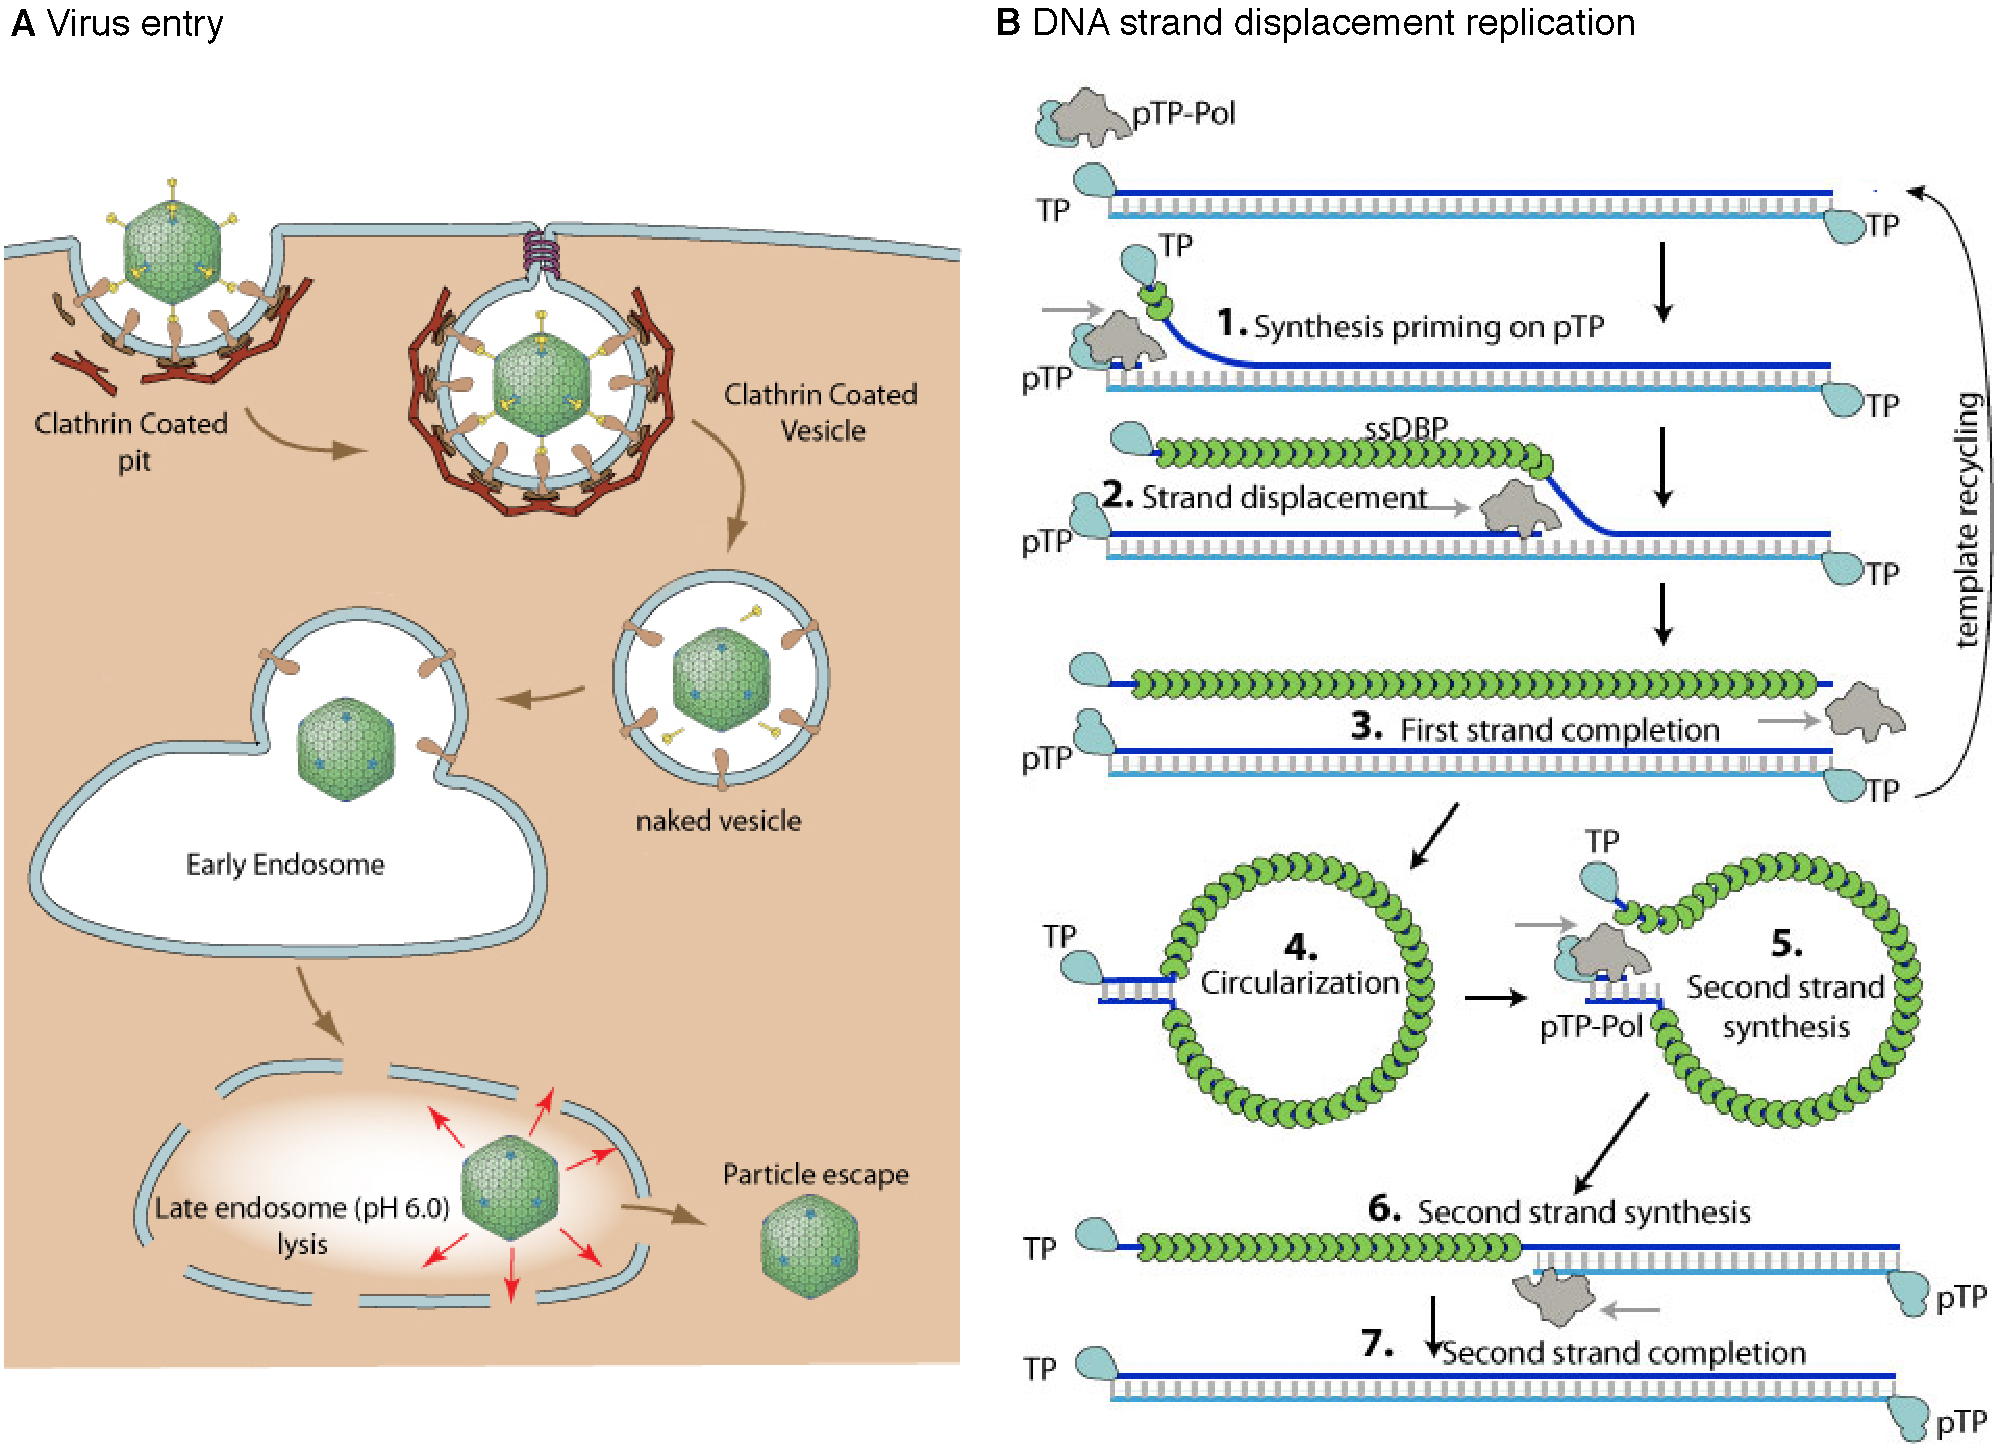
\includegraphics[width=0.95\textwidth]{adenovirus}
  \caption[Molecular mechanisms of adenovirus infection.]{Schematic representation of molecular mechanisms for cell entry and genome replication in adenovirus infection. Formation of the endocytic vesicle is mediated by viral fiber proteins interacting with cellular receptors that in turn recruit clathrin. The \gls{ccp} is pinched off by membrane scission proteins dynamin-1 and dynamin-2, leading to release of a cytosolic \acrshort{ccv} (A). The adenoviral genome is replicated via a mechanism described as DNA strand displacement replication whereby single stranded DNA is synthesized from the viral template in a protein primed fashion, which in turn is copied into double strand DNA. Figures adapted from \cite{Hulo2011}.}
  \label{fig:adenovirus}
\end{figure}

\paragraph{Pathogenesis.}
Initial attachment of virions is mediated by interactions between the globular knobs of viral fiber proteins and target cell \glsrevpl{car}. In \textit{Human adenovirus C} infections, cellular heparan sulfate proteoglycans serve as additional attachment factors, reinforcing adhesion. Subsequent binding of penton bases to \textalpha,\textbeta-integrin receptors induces clathrin-mediated endocytosis and leads to loss of viral fiber proteins (see figure \ref{fig:adenovirus}, A).

The adenoviral replication cycle is divided into early (E) and late stages (L), with each seeing expression of a typical set of genes. Upon engulfment by the host cell and triggered by endosomal acidification, hexon bound protein VI disassociates from the capsid structure and induces lysis of the endosomal membrane. The remainder of the now cytosolic virion is shuttled to the nucleus by microtubular transport where viral protein IX recruits kinesin thereby procuring capsid disruption.

Nuclear penetration is mediated by core protein VII and occurs at \glspl{npc}, leading to transcription of early viral genes by host RNA polymerase II. The resulting proteins manipulate various cellular processes, such as evasion of host immune response (E3, E19), cell cycle (E1A), apoptosis (E1B and E4), autophagy (E1B) and \gls{mrna} transport (E4), while also promoting viral DNA replication (E2). Modulation if the adaptive immune response is mediated by the \gls{tap} inhibitor E19, as binding of \gls{tap} prevents loading of peptides onto \gls{mhc} class I molecules for display on the cell surface. In order to create an optimal environment for replication, viral protein E1A induces a G1\slash S cell cycle transition which increases the concentration of cellular enzymes involved in DNA replication. This, however, also leads to accumulation of cellular p53, participating in apoptosis signaling. Several viral proteins, including E1B 55K and E4 orf6 have been shown to inhibit the apoptotic pathway. E1B 19K is involved in activation of autophagy thereby contributing to the delay or inhibition of apoptosis.

A virally encoded DNA polymerase replicates the genome by DNA strand displacement in an unusual protein primed fashion involving \gls{ptp} acting as primer and \gls{dbp}, stabilizing single stranded DNA, as well as several host proteins (figure \ref{fig:adenovirus}, B). With onset of replication, translation of late genes by host RNA polymerase II is initiated, leading to the production of structural proteins and proteins required for virion assembly. Encapsidation occurs in the nucleus and progeny virions are released by lysis of the host cell.

\paragraph{Epidemiology.}
Adenoviruses are endemic and ubiquitous, causing an estimated 2--5\% of all respiratory infections. Distribution is worldwide and incidence is higher in the first half of the year. Children are frequently infected as serological studies show that by the age of 5 years some 50\% present antibodies towards the most common species, including \textit{Human adenovirus C}. On the order of 1 in every $10^7$ lymphoid cells in the oropharynx harbor fully assembled latent sate virions, making most humans latent carriers. Transmission can both occur via respiratory droplet or fecal-oral routes and virions are very stable towards chemical and physical agents, surviving for long periods outside their host.

Adenovirus outbreaks are a common cause of pneumonia in militaries, leading to the development of live, oral vaccines in the 1960's by the U.S. Army. The only supplier, however, ceased production and as of 1999, vaccinations could no longer be administered, resulting in reemerging incidence. In the first 5 years after loss of the vaccine, 110000 cases of febrile respiratory illness were reported, of which an estimated 90\% are considered preventable. By October 2011, new vaccine again was available and and has been administered to new recruits since.

\subsection{Rhinoviruses}
Investigations into the etiological agent of the common cold within the British Common Cold Research Unit led to the discovery of rhinoviruses in 1953. Initially classified as a separate genus of the family \textit{Picornaviridae}, recent genomic evidence led to a revised taxonomy, recognizing three species of rhinoviruses (A through C) as members of the genus \textit{Enterovirus}. Over 100 distinct serotypes have been isolated from humans, 74 belong to species A, 25 to B and the newly identified species C, currently under active study, may encompass an additional 55 types.

Rhinovirus virions are small (\SI{30}{\nano\meter} in diameter), non-enveloped, with a pseudo $T=3$ icosahedral capsid, consisting of 4 different polypeptides (VP1, VP2, VP3 and VP4) surrounding the RNA genome. There are 60 copies of each structural protein and VP1-3 face towards the outside and are responsible for antigenic diversity, while VP4 faces inwards and anchors the RNA core to the capsid. A canyon formed by VP1 and VP3 serves as receptor binding site. The viral genome consists of monopartite, linear, single stranded, positive sense RNA, roughly \SI{7.2}{\kilobase} in length and encodes a single polyprotein, which cleaved by viral proteases yields 11 proteins. Instead of a methylated 5' cap, the RNA genome is terminated by a viral protein (VPg) at its 5' end \citep{Jacobs2013}.

\paragraph{Diseases.}
Over half and up to two thirds of all cold-like illnesses are thought to be caused by rhinoviruses. In addition, asymptomatic infections, especially in children are very common with rates among children under 4 years ranging from 12 to 32\%. These surprisingly high numbers may to some extent result from virus persistence in hosts that have recovered in addition to disease that has not broken out. In adults, rates of asymptomatic carriage are significantly lower, reported at 0--2\%.

In immunocompetent individuals, symptomatic disease typically manifests as upper respiratory infection with clinical syndromes associated with common cold, including rhinorrhea, nasal congestion, sore throat, headache and possibly fever and general malaise. Disease is self-limited, incubation periods are between 12 and 72 hours and within 7 to 14 days symptoms wear off. A common complication is acute otitis media, which has been reported to happen in up to 30\% of cases in early childhood. In 41--45\% of investigated middle ear infections, rhinoviruses were detected. Further cavities that are frequently infected are the paranasal sinuses. Nose blowing has been suggested as mechanism for spreading the virus and causing rhinosinusitis.

Initially thought to primarily cause benign upper respiratory infections,  recent data clearly implicates rhinoviruses in more severe lower respiratory infections. Croup, bronchiolitis and \gls{cap} have been associated with rhinovirus infections and studies have shown that in 12--26\% of cases, rhinoviruses were present. Furthermore, a study of children admitted to \glspl{icu} with lower respiratory tract infections detected no other pathogens in 49\% of the patients. Immunocompromised individuals are predisposed to contracting more serious forms of disease, with morbidity and mortality comparable to that of pandemic H1N1 influenza.

While not typically associated with cytopathogenic effects on epithelia of the upper respiratory tract, cell damage to lung tissue, especially among children, has been documented. Thus, rhinoviruses are linked to exacerbations of chronic pulmonary diseases such as asthma, chronic obstructive pulmonary disease and cystic fibrosis.

\begin{figure}
  \centering
  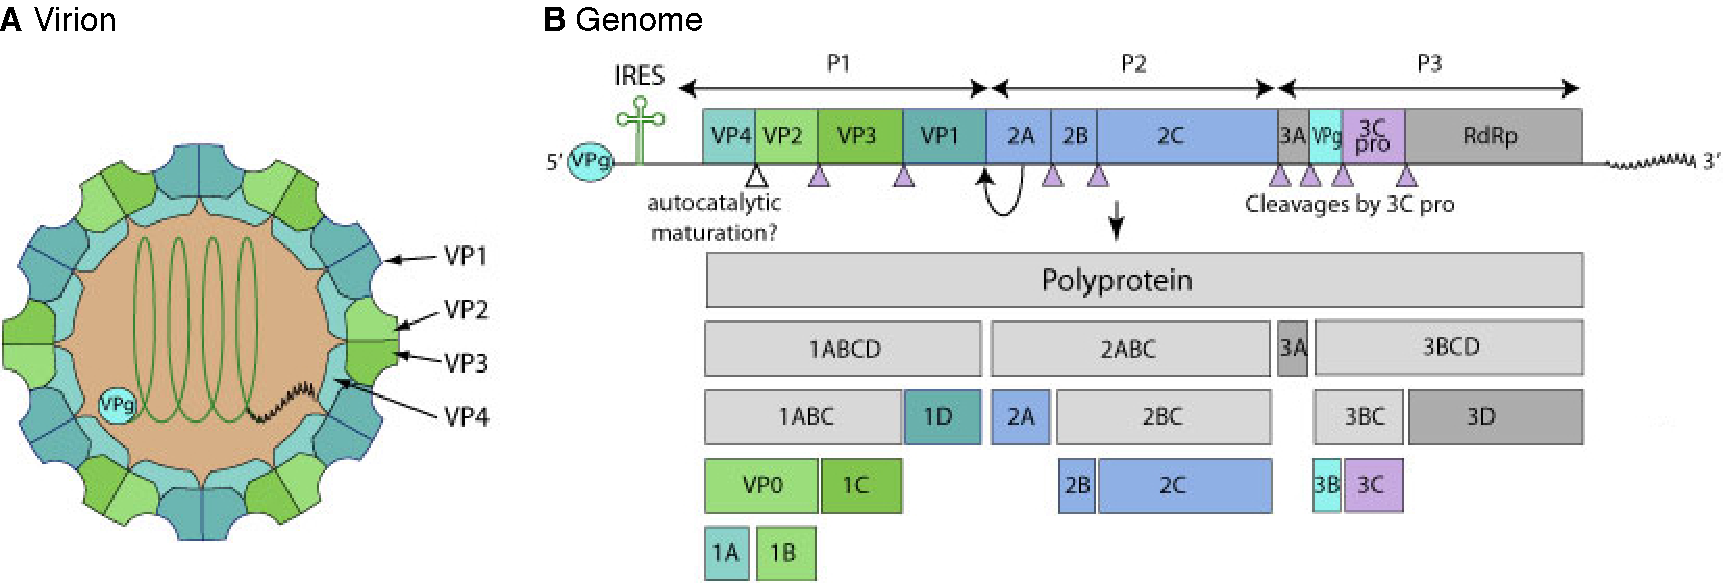
\includegraphics[width=0.95\textwidth]{rhinovirus}
  \caption[Capsid structure and genome of rhinoviruses.]{Capsid proteins VP1 through VP4 form a pseudo $T=3$ icosahedral coat, roughly \SI{30}{\nano\meter} in diameter around the RNA genome (A), which is monopartite, linear, \SI{7.2}{\kilobase} long and encodes 11 proteins (B). Figures adapted from \cite{Hulo2011}.}
  \label{fig:rhinovirus}
\end{figure}

\paragraph{Pathogenesis.}
Members of rhinovirus species A and B are divided into two group according to their host cell receptors. Members of the major group form interactions with \gls{icam-1} while minor group types (including serotype 1a) associate with \glspl{vldlr}. Attachment of species C have very recently been identified as induced by \gls{cdhr3}. Upon receptor mediated endocytosis, pH dependent conformational changes in capsid structure exposes VP4 which has pore-forming properties and facilitates release of viral genomic material into the cytosol.

Host cell ribosomes readily translate the released positive-sense RNA into polyprotein, which is cleaved in \textit{cis} by 2A and 3Cpro, yielding preproteins P1, P2 and P3 (see figure \ref{fig:rhinovirus}. P1 is digested into structural capsid proteins while P2 and P3 are further processed to produce the replication machinery. Viral RNA-dependent RNA polymerase synthesizes a complementary, negative-sense RNA strand, primed by VPg, which in turn serves as template for many copies of the viral genome. These can be both translated into more protein and in a later stage of replication also be packaged into progeny virions. Final cell export is mediated by host-cell membrane lysis.

\paragraph{Epidemiology.}
Despite most infections with rhinoviruses only resulting in mild disease, economic impact both due to health care costs and loss of productivity is considerable. This is primarily owed to the overwhelming prevalence of these pathogens. Respiratory illnesses attributed to rhinoviral infections occur throughout the world and all year round with peak incidences in early fall and spring. Vaccination efforts so far have been futile, mainly because of the large number of serotypes and lack of individual epidemiological data.

Due to acid-sensitivity, fecal-oral infection is unlikely most person-to-person transmission occurs through aerosols and contact spread either direct of via fomites. Extra-host survival times of hours to days have been reported for indoor environments and up to 2 hours on undisturbed skin.

\subsection{Vaccinia}
\textit{Vaccinia virus} is a species within the genus \textit{Orthopoxvirus}, alongside the exceptionally virulent \textit{Variola virus}, the etiological agent of smallpox. Immunological similarities between the two species allows for cross-protection, which coupled with the large discrepancy in pathogenicity presents a fortunate opportunity for artificially inducing acquired immunity. This was recognized by Jenner in 1798, while investigating the zoonosis of \textit{Cowpox virus} and subsequent susceptibility towards contraction of smallpox. The origins of vaccinia are unknown. It has been speculated to have derived from cowpox or smallpox, to be a hybrid of both and of being the prototype orthopoxvirus, as well as descending from an extinct ancestor.

The virions are large and brick shaped, measuring 200 by 250 by \SI{340}{\nano\meter} and exist as both \gls{mv} and \gls{ev}. Structurally they are unusually complex. The linear, double-stranded DNA genome, roughly \SI{200}{\kilobase} long, is encased in an S-shaped, tube-like nucleocapsid with an outside diameter of \SI{50}{\nano\meter}, a cavity of \SI{10}{\nano\meter} and an overall length of \SI{250}{\nano\meter}. Additionally, 47 viral proteins, of which 16 are involved in early \gls{mrna} synthesis and 28 have no known enzymatic function, are packed into a core structure. The core wall consists of two layers, the palisade (outer) layer which is \SI{17}{\nano\meter} thick and an inner smooth layer, measuring \SI{8}{\nano\meter} across. Centered on the top and bottom faces, two proteinaceous lateral bodies separate core from the surface membrane, forming the virion core into a biconcave disc with dumbbell shaped vertical cross sections. The lipidic surface membrane also consist of two layers, the outermost measuring \SI{9}{\nano\meter} and the innermost domain is \SI{5}{\nano\meter} thick. \Gls{ev} virions are additionally wrapped in a membrane derived from Golgi cisternae \citep{Marennikova2005,Condit2006}.

\paragraph{Diseases.}
While infection with variola causes severe disease manifesting in skin lesions covering the whole body, accompanied by 20--40\% mortality rates, the closely related \textit{Vaccinia virus} is far less invasive. Virulence of the latter pathogen is so low that it has been routinely used as live vaccine against the former. Owing to the massive effort put into the worldwide fight against smallpox led by the \gls{who} in the late 1960's and throughout the 1970's, the disease was found to be eliminated by 1980. At the center of the smallpox eradication program was the administration of freeze-dried, calf lymph derived vaccinia with a bifurcated needle, by multiple pricking of the skin. Towards the end of the initiative, 200 million vaccinations were performed annually.

The predominant reaction to vaccinia inoculation is localized, self-limited disease. After an incubation period of of 3--4 days, a papule with a sunken center develops at the site of infection, accompanied by erythema and swelling. Over the following days the papule increases in size and liquid begins to accumulate within. Fever may develop around days 7--10, possibly followed by malaise, headache and anorexia. Local lymphadenopathy is frequently encountered and days 8--10 typically mark the beginning of involution of the papule, which subsequently drys out and forms a scab.

Of great concern for routine vaccination procedures are complications which inevitably occur in a small numbers. Atypical side effects develop in roughly 1 per mill of cases and potentially life threatening reactions usually manifest as neurological (477.4 cases and 47.0 fatalities per 1 million) or cutaneous disease (278.4 cases and 0.2 fatalities per 1 million). Predisposing conditions for central nervous system involvement are not known and despite decades of inquiry into this pathology, it remains poorly understood. Symptoms range from febrile seizures to severe encephalitis, but so far no  neuropathological characteristics have been identified. Complications affecting the skin and mucous membranes are classified as progressive vaccinia, eczema vaccinatum and generalized vaccinia and disease severity decreases in this order. Predisposing conditions for progressive and generalized vaccinia are immunodeficiencies while a history of eczema is a risk factor for eczema vaccinatum.

\begin{figure}[t]
  \centering
  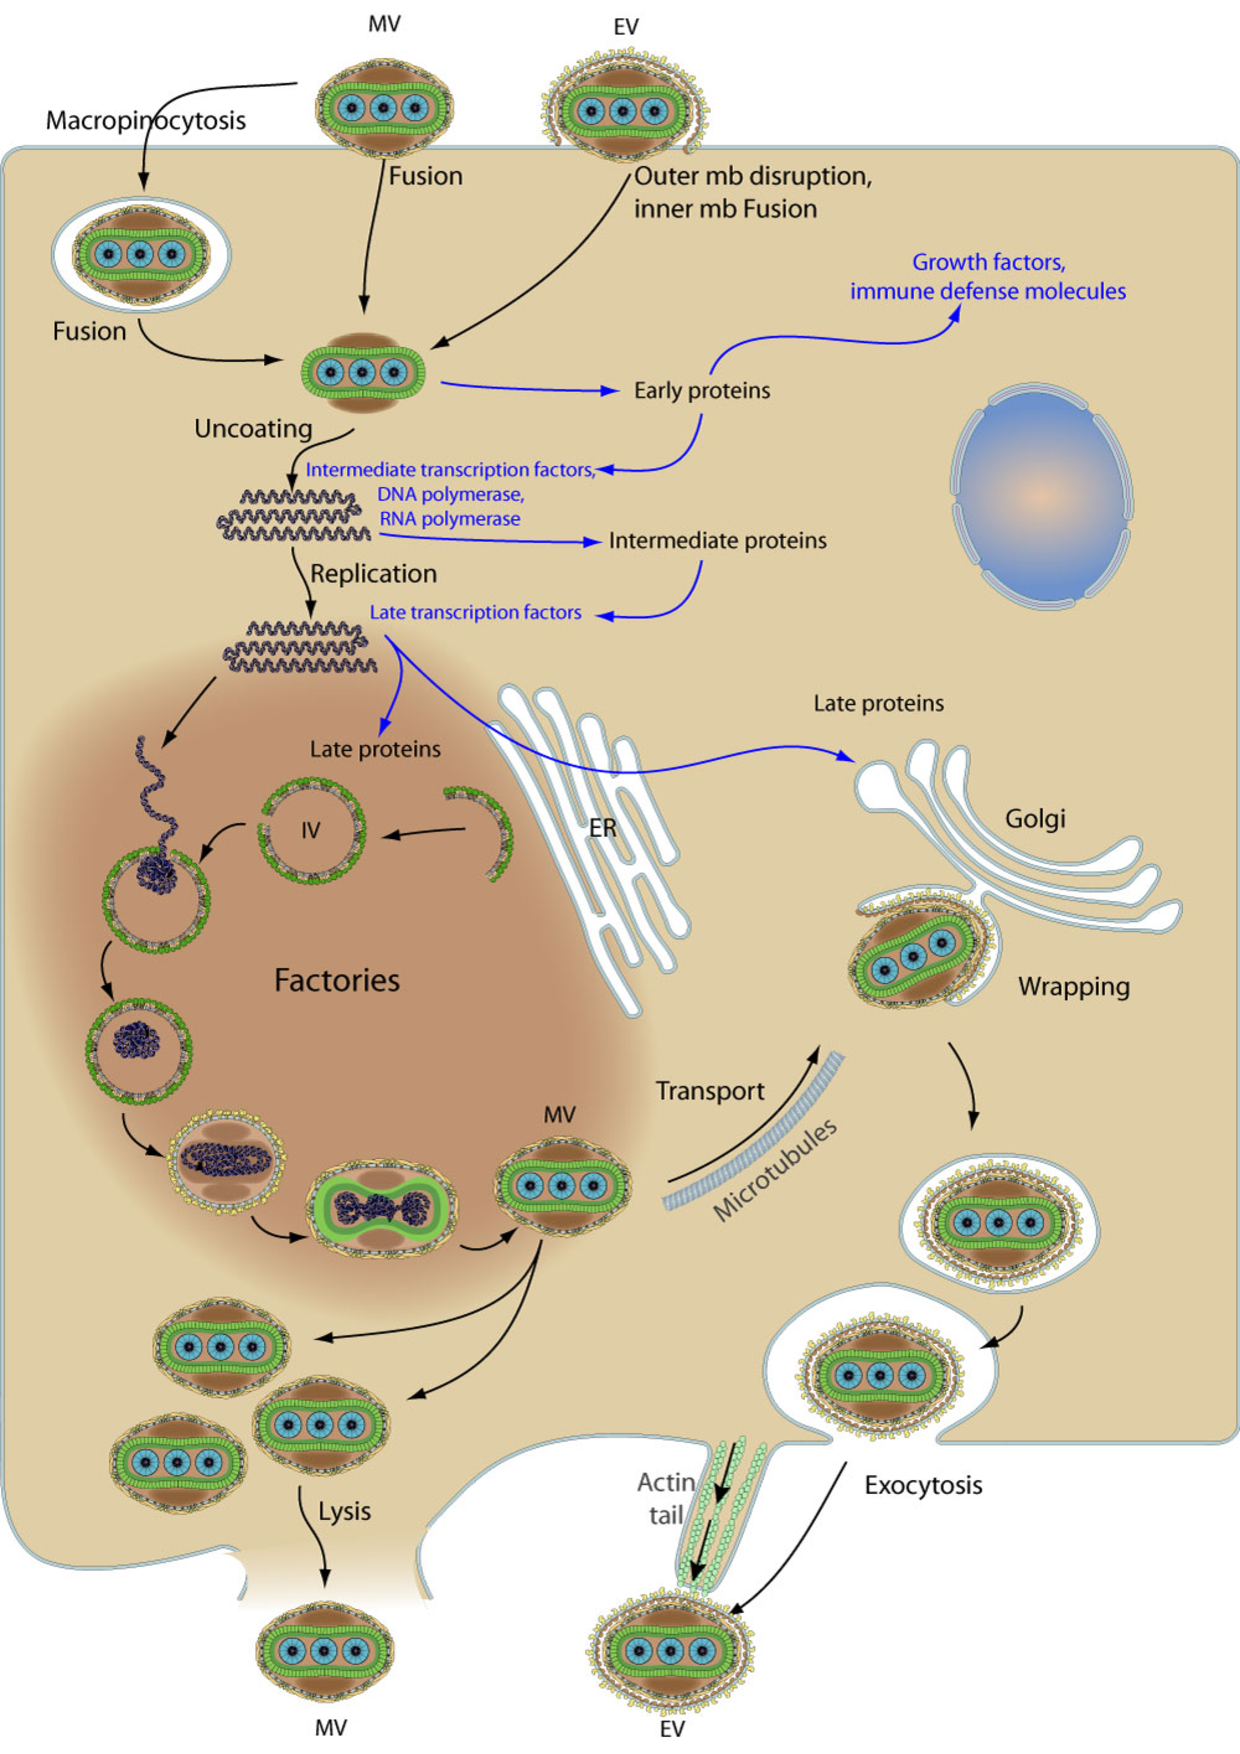
\includegraphics[width=0.75\textwidth]{vaccinia}
  \caption[Replication cycle of \textit{Vaccinia viruses} for both intracellular mature and extracellular enveloped virions.]{Replication cycle of \textit{Vaccinia viruses} for both \acrfull{mv} and \acrfull{ev}. Cell entry is either macropinocytic or proceeds via membrane fusion, followed by uncoating and replication. Host exit proceeds by either lytic or exocytic mechanisms. Figure adapted from \cite{Hulo2011}.}
  \label{fig:vaccinia}
\end{figure}

\paragraph{Pathogenesis.}
Initial attachement is mediated by interaction between viral proteins and cellular heparan sulfate chains. For cell entry, various strategies have been reported, depending on the strain under investigation. WR strains induce macropinocytosis and proteins A25\slash A26 act as fusion suppressors that only lift their embargo under acidic conditions encountered in a maturing endosome, while other strains, such as Copenhagen, present no A25\slash A26 on their outer membrane and fuse directly with the target plasma membrane. Due to the additional membrane of \glspl{ev}, a differing entry mechanism needs to be employed. In a currently not well understood fashion, the outer membrane is lost by non-fusogenic disruption, followed by fusion of the inner virion membrane. All pathways lead to cytosolic localization of virions devoid of their envelope (c.f. figure \ref{fig:vaccinia}).

Members of the \textit{Poxviridae} family are special among Baltimore group I viruses in that their genome encodes all necessary replicatory proteins, allowing for cytosolic localization. Replication is temporally tightly regulated and consists of distinct phases of early, intermediate and late gene expression. Each class of genes encodes factors capable of initiating the succeeding stage, providing transcription level regulation. Uncoating of the core structure releases early proteins, including RNA polymerases and enzymes for \gls{mrna} processing which start transcribing early genes. At least 50 different products, such as DNA replicatory enzymes, additional RNA polymerase, \gls{mrna} processing machinery, host defense molecules and intermediate gene transcription factors, have been identified and account for 25\% of the viral coding capacity. Early gene transcripts are detectable 20 minutes after cell entry and reach their productive peak within 100 minutes of infection.

Expression of intermediate genes is initiated by accumulation of intermediate  transcription factors and the onset of DNA replication. Only 7 products of this phase are known, which functionally are mostly concerned with host defense, DNA\slash RNA metabolism and commencement of the final phase. Beginning 100 minutes after infection, intermediate gene transcription reaches its peak at 120 minutes and is thereafter superseded by late gene transcription, beginning 140 minutes after cell entry. Products of the final phase comprise a large number of genes (up to 75\% of the vaccinia genome) and include enzymes needed for initiating replication (RNA polymerase and modification proteins), early transcription factors and structural proteins, as well as virion assembly machinery.

DNA replication not only serves for progeny virions, but also to increase the concentration of templates used for gene expression. Both DNA synthesis and virion assembly occur within factories, readily visualized by electron microscopy as electron dense cytoplasmic inclusion bodies. Owing to the complex virion structure DNA packaging and virion assembly is an involved procedure with is incompletely understood.

\paragraph{Epidemiology.}
It is unknown if a natural reservoir of vaccinia exists. It has been speculated that the virus is maintained only within research laboratories and vaccination production facilities, while others have implicated some rodent species as possible reservoir hosts. Small scale zoonotic outbreaks of vaccinia have been documented in Brazil and it was initially suspected that these were linked to vaccine that had escaped into the environment. Recent phylogenetic studies however were able to rule out this explanation but were unable to shed further light into underlying epidemiological mechanisms.

While transmission from vaccinees to unvaccinated individuals is rare, direct contact transmission is possible and such occurrences have been documented. Special care has to be taken to avoid direct contact between recently vaccinated and individuals predisposed towards developing complications.

\section{RNA Interference}
First described only two decades ago, regulation of gene expression by short strands of RNA has become an indispensable tool to both experimental biology and bioinformatics. Recognizing the importance of applications made possible by this discovery, the 2006 Nobel prize in Physiology or Medicine was awarded to Fire and Mello who studied RNA interference in the nematode worm \textit{Caenorhabditis elegans} and published their findings in 1998. Building on studies by Guo and Kemphues, who showed that sense RNA, as well as antisense RNA was capable of suppressing gene expression, Fire, Mello and coworkers found that double stranded RNA was at least ten-fold more effective as silencing agent than individual single stranded fragments. Further investigations showed that several gene regulatory processes, previously thought to be unrelated, were in fact manifestations of RNA interference and that the underlying mechanism was conserved in many, if not most, eukaryotic organisms \citep{Hannon2002}.

The RNAi pathway can take as input two separate types of RNA molecules, \gls{mirna} and \gls{sirna}, of differing origins. While \glspl{mirna} are endogenous and purposively employed in post-transcriptional regulation of gene expression, \glspl{sirna} are exogenous synthetic or viral inducers of gene suppression, in which case, RNA interference can be viewed as an immune response to foreign genetic material. Parsimony-based phylogenetic analysis of involved genes suggests that the key components to an RNAi system were already present in the last common ancestor of eukaryotes and were subsequently lost or extensively simplified in some protists. The original function of RNAi is hypothesized to be that of a defense mechanism against genomic parasites as indicated by the extent of its conservation, whereas \gls{mirna}-directed silencing most probably was introduced at a later point in evolution \citep{Cerutti2006}.

\subsection{Molecular Mechanism\footnote{This section is based on the three review articles by \cite{Wilson2013}, \cite{Kim2007} and \cite{Carthew2009}.}}
RNA interference refers to three separate mechanisms for regulation of gene expression by small RNAs, as visualized by figure \ref{fig:rnai}. While \glspl{sirna} are involved both in transcriptional and post-transcriptional gene silencing, the \gls{mirna} pathway is focused on translational repression. The severity of action on the targeted genes once again highlights the differing purposes of the \gls{sirna} and \gls{mirna} pathways, one tasked with inhibitory and the other with regulatory measures.

\begin{figure}[t]
  \centering
  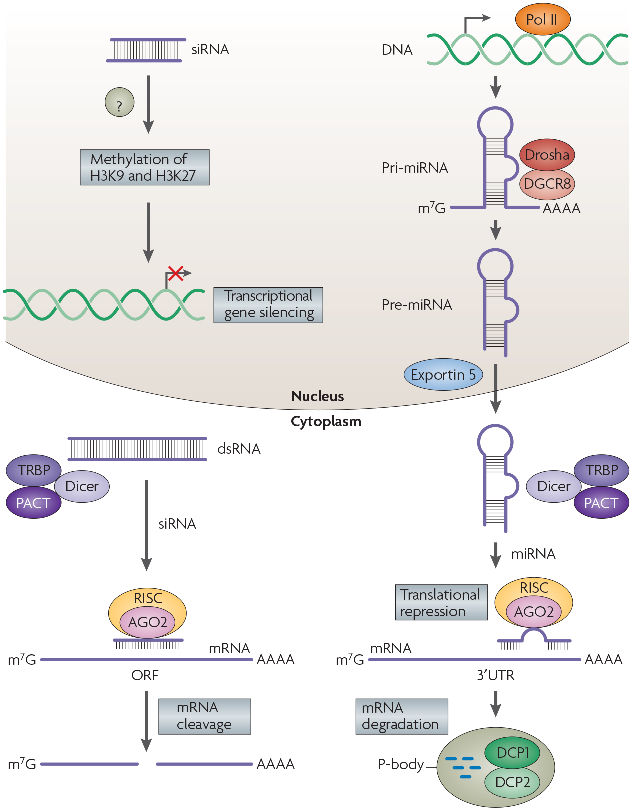
\includegraphics[width=0.7\textwidth]{rnai}
  \caption[The three major pathways of RNA interference.]{RNA interference comprises of three distinct mechanisms that yield control over gene expression. Exogenous double-stranded RNA are processed into \gls{sirna} fragments that both act inside the nucleus as transcriptional silencing agents and in the cytoplasm, post-transcriptionally cleaving \gls{mrna} strands. Endogenous \gls{mirna} is synthesized by RNA polymerase, originates from the nucleus in processed form and mediates milder translational repression Figure adapted from \cite{Kim2007}.}
  \label{fig:rnai}
\end{figure}

\paragraph{Translational repression by \gls{mirna}.}
The biogenesis of \gls{mirna} occurs in the nucleus and is initiated by RNA polymerase II transcription of long (\textgreater \SI{1000}{\nucleotide}) \gls{pri-mirna} segments, characterized by double-stranded hairpin loops with single-stranded 5'- and 3'-terminal overhangs which are polyadenylated and capped. Subsequent processing by the microprocessor complex consisting of the RNase III family enzyme Drosha and \glsrev{dgcr8} yields \tilde 60--\SI{70}{\nucleotide} stem-loop structured \gls{pre-mirna} fragments. \gls{dgcr8} recognizes \glspl{pri-mirna} by the junction of stem and single-stranded overhang and helps positioning the substrate for endonucleolytic cleavage by Drosha at a site \tilde \SI{11}{\nucleotide} from the junction. Nuclear export is mediated by the transport facilitator exportin-5 and is Ran-GTP dependent.

In the cytoplasm, \glspl{pri-mirna} are targeted by Dicer and the associated dsRNA binding proteins \glsrev{trbp} and \glsrev{pact} for further processing into 21--\SI{25}{\nucleotide} dsRNA strands with \SI{2}{\nucleotide} overhangs at the 3' termini and phosphate groups at each of the recessed 5' ends. The mature \glspl{mirna} are loaded onto \gls{ago} by Dicer, which leads to the formation of \gls{risc}. Concomitantly with \gls{risc}-loading, one of the two RNA stands is selected as guide strand whereas its complement (the passenger strand) is ejected and degraded. Thermodynamic asymmetry between the two strands is exploited in this step and the strand with the less stable 5' end is preferred. As opposed to strand separation in \glspl{sirna}, the passenger strand is not cleaved but rather unwound by helicase activity, facilitated by imperfect sequence alignment.

Finally, active \gls{risc}, exposing the \glsdesc{ago}-bound guide strand, interacts with the 3' untranslated region of \gls{mrna} targets and directs translational repression and \gls{mrna} degradation. Sequence homology between \gls{mrna} and the \gls{mirna} seed sequence (the first 2--6 or 2--\SI{8}{\nucleotide} from the 5' end) is critical while mismatched nucleotides towards the 3' end of the \gls{mirna} are readily tolerated. The extent of base-pairing influences the subsequent mechanism of silencing, ranging from direct target cleavage (perfect match) over deadenylation (followed by degradation) to nonendonucleolytic translational repression (imperfect match).

\paragraph{Post-transcriptional gene silencing by \gls{sirna}.}
Precursors to \gls{sirna} are long, linear, perfectly base-paired double stranded sequences of RNA, typically of exogenous origin either introduced directly into the cytoplasm, or taken up from the environment. A complex consisting of Dicer and several RNA-binding proteins are responsible for trimming down dsRNA fragments to the appropriate size for loading onto \gls{ago}2. Of the four \glsdesc{ago} family members in humans, capable of associating with \gls{mirna}, only \gls{ago}2 seems to be involved with \gls{sirna}. Furthermore, \gls{ago}2 is the only mammalian \glsdesc{ago} bearing endonucleolytic functionality and therefore capable of directly cleaving targeted \gls{mrna}.

Strand selection is again based on differences in stability of base-pairing at the 5' termini with the weaker interacting end being favored as guide strand. Accuracy of discrimination can be low, leading to incorporation of both strands with equal frequency. In contrast to \gls{mirna} loading, the passenger strand is not merely separated but directly cleaved by \gls{ago}2 and the differing treatment seems to only depend on perfect strand complementarity given in \gls{sirna} and absent in \gls{mirna}. Upon RNA incorporation, \gls{risc} is formed and activated by cleavage of the passenger strand. The 3' guide strand end is bound by the \glsdesc{ago}'s \gls{paz}, while the 5' end interacts with \gls{mid}, closely located to the catalytic RNase H-like \gls{piwi}.

Post-transcriptional gene silencing is accomplished by endonucleolysis of perfectly matching \gls{mrna} precisely at the phosphodiester linkage between bases 10 and 11 relative to the 5' terminus of the \gls{sirna} guide strand. Following cleavage, the target disociates, freeing \gls{risc} for further catalysis, and the \gls{mrna} fragments are degraded by cellular exonucleases. Imperfectly matched \gls{mrna} may be targeted, much like it is the case with \gls{mirna}, leading to \gls{sirna} off-target effects which are of great practical importance.

\paragraph{Transcriptional gene silencing by \gls{sirna}.}
In addition to post transcriptional action of \gls{sirna}, nuclear inhibition of gene transcription has been described in many eukaryotes. Diced \gls{sirna} fragments are transported into the nucleus where they are assembled with a group of proteins, including \gls{ago}1, to form \gls{rits}. Currently only incompletely understood, the \gls{sirna} guide strand is thought to recognize RNA transcripts as the emerge from RNA polymerase II, followed by recruitment of factors that enable covalent modifications of nearby histones. Methylation of lysines 9 and 27 in H3 by histone methyltransferases leads to chromatin compaction and heterochromatin formation. \Gls{rits} has also been shown to induce direct methylation of DNA, repressing gene expression even further.

Contributing to the potency of RNA interference, engagement of \gls{rits} with nascent transcripts activates the \gls{rdrc}, capable of generating secondary \gls{sirna} fragments and therefore amplifying silencing capabilities. The role of this reinforcement mechanism has been firmly established in many eukaryotic RNAi systems with the notable exceptions of vertebrates and insects. Whether a similar system exists in these organisms remains an open question.

\subsection{Biological Function}
The mechanisms of RNA interference have most probably evolved in order to protect against foreign genetic material such as parasitic DNA sequences or viral RNA. Transposable elements (transposons) are DNA sequences that are mobile within the genome, can make up a significant fraction of eukaryotic genomes and are typically considered non-coding. Transposition is mediated by transposases, enzymes often encoded within the transposons themselves, that act on specific sequences at the transposon ends and cause unspecific insertion into new target sites. Retrotransposons move via an RNA intermediate which is reverse transcribed to DNA and inserted, while DNA transposons employ a cut and paste mechanism. Retroviruses therefore can be viewed as transposons and in general, transposable elements are a form of selfish DNA that often incur deleterious effects.

RNAi is an important regulatory force to transposon activity, both by processing transcripts of retrotransposons, thereby reducing their concentration and eliciting epigenetic modifications, as well as transcriptional inhibition via heterochromatin formation. The importance of keeping transposable elements in check is highlighted by their prevalence, with roughly half of the human genome being thought to derive thereof.

Antiviral mechanisms are particularly important in organisms lacking an adaptive immune system as found in vertebrates and exploiting the orthogonality of most genomic systems to double-stranded RNA puts RNA interference in a powerful position. Corroborating this notion is the observation that, in \textit{Drosophila melanogaster}, three key proteins of the RNAi pathway (Dicer-2, \gls{ago}2 and R2D2, a protein involved in \gls{risc} loading) are among the top 3\% in terms of genetic instability. Furthermore, \gls{mirna} pathway paralogs to these three genes (Dicer-1, \gls{ago}1 and R3D1), not being involved in immune response, evolve at a much slower rate \citep{Obbard2009}.

Although small RNA-guided, \gls{ago}-dependent up-regulation of gene expression (termed RNA activation or RNAa) has been described, most regulation of gene expression by \gls{mirna} is of inhibitory nature. This widespread mechanism, consisting of \textgreater 1000 \gls{mirna} sequences (as much as 5\% of the human genome) controls at least 30\% of human genes and is responsible for vital processes including cell growth, tissue differentiation and cell proliferation.

\subsection{Applications}
In \textit{C. elegans}, RNA interference is especially powerful, making it a popular model organism for RNAi. Not only is delivery efficiently possible simply by feeding the nematodes with bacteria such as \textit{E. coli} that carry the desired dsRNA, but the resulting gene silencing effects are hereditary. Moreover, RNAi response is not stoichiometric but catalytic, is amplified in a feedback loop and in many organisms, systemic spread has been documented.

The initial burst of excitement surrounding possible applications was somewhat moderated by difficulties in applying RNAi to mammalian systems. At first it seemed impossible to use this technology in somatic cells as the introduction of dsRNA is typically met with overwhelming non-specific responses, including  \gls{pkr}, which leads to arrest of translation and apoptosis. This issue was shown to be overcome by exclusively using \glspl{sirna} duplexes of 21--\SI{23}{\nucleotide} with 2-nt 3' overhangs that mimic Dicer products and are too short for inducing \gls{pkr}. Mammalian RNAi response, however is transient, lacking amplification and spreading mechanisms documented in other organisms (mainly plants and worms) and delivery, especially in vivo remains problematic. A further issue that continues to be an actively researched area of interest is that of \gls{ote}, which considerably complicate the interpretation of phenotypic data.

\paragraph{Gene knockdown studies.}
Large-scale \gls{lof} and modifier or synthetic lethality screens are readily possible by means of RNAi based \gls{hts}. Such experiments usually proceed by arraying libraries of gene specific \glspl{sirna} onto microtiter plates (96 and 384 well formats are common), followed by the addition of liquid cell cultures. After an appropriate transfection time, the cells may be subjected to an additional treatment, such as exposure to drugs or pathogens (modifier screen) or \gls{lof} phenotypes can be investigated directly. Assay readout is performed via optical measurements such as detection of fluorescence or luminescence signals or by microscopic imaging (confocal or wide-field).

Transcriptional reporters, fluorescent dyes that detect enzymatic activity and protein-modification specific antibodies have been employed in plate reader-based investigations which yield a single numerical readout per well. This quantitative approach is contrasted with microscopy based assay read-outs that are able to capture spatial information on antibody stained proteins, fluorescently labeled cellular structures and \gls{gfp} expression, yielding much more data per well. Significant challenges incurred by automated high-content imaging have successfully been addressed by computational image analysis software.

A multitude of sources of technical and biological noise contribute to serious problems in interpretability and comparability of observed data. Common to all high throughput approaches, errors arise from difficulties guaranteeing equal conditions in a large number of parallel experiments. Liquid dispensing errors, temporal disparities caused by bottleneck resources such as imaging equipment and spatial discrepancies, for example inhomogeneous temperature distribution over the plate or liquid evaporation in border wells, are only a few issues that come to mind. Biological sources of error include \glspl{ote}, varying potency of reagents (both the knockdown strength and time required to achieve optimal knockdown may be affected) and obscuration of assay phenotype by the knockdown phenotype (e.g. cell death). Furthermore, incorrect gene models lead to errors in library design and detection may be hampered by weak phenotypes. Replicates, although expensive in large-scale experiments and control wells embedded in every assay plate are indispensable measures in order to assess reproducibility of the data \citep{Echeverri2006,Perrimon2007}.

Despite being a young technology, RNA interference has already proven itself as an invaluable tool and has yielded many insights with significant impact on various fields. A review by \cite{Mohr2010} lists some of these findings which lead to refined understanding of cell proliferations, cancer biology, cell cycle regulation, mitochondrial diseases, signal transduction, RNA biology and pathogen response. 

\paragraph{Biotechnological applications.}
Intercellular, systemic spread of RNAi response in plants and even its heredity over several generations have been documented and it comes as no surprise that the technology is investigated for possible utilization in crop improvement. Removal of plant endotoxins by targeting genes of toxin biosynthesis has been accomplished, leading to the production of decaffeinated coffee plants (knockdown of theobromine synthase), tobacco with reduced concentration of carcinogenic compounds (inhibition of nicotine demethylase activity) and edible cotton seeds (reduction of delta-cadinene synthase leads to low levels of gossypol, a toxic terpenoid), which are naturally rich in dietary protein.

In addition to investigations with consumer health in mind, improvements in environmental resistance have been studied in many organisms. Susceptibility to bacterial and viral pathogen infection has been reduced in rice, bean, barley and lemon, while fungal resistance has been increased in potato, tobacco and wheat. Successful RNAi application as insecticide has been shown in cotton and maize and even improved resistance to parasitic weeds could be demonstrated in transgenic tomato plants. Despite these achievements, concerns over environmental issues and adverse health effects have so far prevented RNAi based genetic modifications from exiting experimental stages \citep{Saurabh2014}.

\begin{table}
  \centering
  \caption[A selection of RNAi based drugs in clinical trials.]{A non exhaustive list of RNAi based drugs that currently are in clinical trials. The data was obtained from the clinicaltrials.gov database \cite{McCray2000}}
  \label{tab:rnai-clinical}
  \footnotesize
  \begin{tabular}{L{0.14\linewidth}L{0.24\linewidth}L{0.24\linewidth}L{0.18\linewidth}}
    Company &
      Disease &
      Delivery system &
      Status \\
    \hline 
    Alnylam &
      (TTR)-Mediated Amyloidosis &
      siRNA–GalNAc conjugate &
      Phase III recruiting \\
    Alnylam &
      Antitrypsin Deficiency Liver Disease &
      Liposome &
      Phase II recruiting \\
    Alnylam &
      Acute Intermittent Porphyria &
      siRNA–GalNAc conjugate &
      Phase I recruiting \\
    Silenseed &
      Advanced pancreatic cancer &
      Polymer (LODER) &
      Phase III planned \\
    Sylentis &
      Dry eye syndrome &
      Naked \gls{sirna} &
      Phase II completed \\
    Sylentis &
      Open angle glaucoma &
      Naked \gls{sirna} &
      Phase II recruiting \\
    Tacere &
      Chronic hepatitis C &
      \gls{aav} vector &
      Phase II recruiting \\
    Tekmira  &
      Advanced Hepatocellular Carcinoma &
      Liposome &
      Phase II recruiting \\
      \hline
  \end{tabular}
\end{table}

\paragraph{Therapeutic potential.}
Great promise lies in therapeutic application of RNAi as theoretically, any gene can be targeted, yielding unparalleled flexibility not encountered with typical small molecule drugs. An initial obstacle to harnessing this power in humans is the issue of delivery. Systemic spread of naked \glspl{sirna} is hampered by kidney filtration, phagocytic uptake and degradation by serum RNases. Movement across capillary walls is not readily possible for molecules larger than \SI{5}{\nano\meter} and phagocytes patrol the extracellular matrix, ingesting foreign genetic material. Furthermore, polyanionic macromolecules do not easily penetrate hydrophobic cellular membranes.

Topical or local administration offers advantages, including increased bioavailability and reduced side effects and is therefore preferred for treatment of eye, skin and mucosal diseases, as well as localized tumors. If targets are not localized or difficult to reach, injection into the bloodstream may provide a mode of systemic application. Chemical modification of the RNA backbone (2'-O-methylation or 2'-fluorination of ribose) has been shown to provide resistance to RNase and covalent attachment to cholesterol promotes cellular uptake. Encapsulation of \gls{sirna} in liposomes and cationic polymers are further proven techniques for improving extracellular stability, stimulate endocytosis and facilitate endosomal escape.

Some sort of target selectivity is desirable on order to avoid high dosages, associated concerns of toxicity and potential \glspl{ote} in non-target tissue. Coupling of \gls{sirna} reagents to antibodies specific for \gls{hiv} envelope glycoproteins has been successfully employed for selectively entering infected cells, while aptamers (oligonucleotides specifically engineered for binding a given target), carrying \glspl{sirna} have also been shown to be capable homing mechanisms.

Viral delivery of of RNAi inducing agents presents an alternative technique to the above and in case of retroviral transport vessels, \glspl{shrna} that are reverse transcribed and integrated into the host genome, provide stable expression and prolonged RNAi activity. Adenoviral and \gls{aav} vectors have also been employed, resulting in a more transient response. While health concerns associated with perpetuity of gene therapy no longer apply, repeated administrations may prove problematic, triggering strong immune response and thereby limiting therapeutic potential.

Currently, multiple \gls{sirna} based therapeutics are in clinical trials, including stage III studies (see table \ref{tab:rnai-clinical}). Due to the unprecedented pace at which RNAi technology went from discovery to development of applications, much uncertainty remains surrounding long term effects of exposure to such drugs. Chronic diseases including hepatitis C or \gls{hiv} infections require life-long treatments and consequences of repetitively triggering RNAi response has not been thoroughly studied (unwanted changes to chromatin structure for example, are one area of concern). Apart from safety issues, several implementation aspects require further study. While neurodegenerative diseases have successfully been treated in mouse models via direct injection into the brain, this is not easily feasible in human patients and currently no delivery vehicle capable of crossing the blood-brain barrier. \citep{Kim2007,Whitehead2009},
